
%\chapter{Vision, Action and World Models}\label{chap:world}
\chapter{Vision, Action and World Models}\label{chap:world}

\begin{learningbox}
Agents act in a world that consists of more than language. In this chapter you will learn how  transformer-based models can gain world knowledge in modalities beyond language.
Specifically, you will be able to:
\begin{itemize}[leftmargin=*, nosep]
    \item Describe the architecture of {\em vision-language models}, or VLMs, (mostly) transformer models  that consist of a language and a vision part. VLMs are highly successful, for example in generating realistic fake images, and film clips. 

    \item Understand how {\em vision-language-action} models work. VLAs are also trained on robotic action. VLAs help improve the generality of robot behavior.
    
    \item Explain why agents benefit from {\em world models}: models that have learned some physical aspects of the world around us, preventing  agents from attempting to walk through walls. %The term {\em world model} is borrowed from the field of {\em model-based reinforcement learning}, where such models are trained from observations in the environment, and then used to efficiently learn optimal action policies.  
\end{itemize}
\end{learningbox}


%*
%- pretraining
%-- vlm
%-- decisions
%-- VLA
%- finetuning
%-- decisions
%-- action

%- vlm
%-- pretraining
%-- finetuning
%- decisions
%-- pretraining
%-- finetuning
%- VLA
%-- pretraining
%-- finetuning

%Todo: read Ch 7 and write contents

%benchmark
%architecture
%learning/code
%results
\begin{comment}
    
%
Agents act, and the LLM should do the reasoning for these actions. To do so, the LLM needs to understand more than just  language. For example, a robotic agent needs to understand which joints to move in its arms. Furthermore, agents may need to be able to interpret spatial or visual data. 

The previous chapter discussed  approaches to improve LLM reasoning by in-context methods. %, a powerful and efficient learning method that does not change the parameters of the underlying transformer model.
%
%, but works purely at the prompt level at inference time. 
To learn other modalities than language, we have to pretrain and finetune the models: we need to go beyond what is possible by in-context learning. 
% , where we do train the parameters of the transformers. 

In this chapter we will shift our focus from language to vision and actions, and our learning methods from in-context learning to  pretraining and finetuning. 
\end{comment}

\section{Multi-modal Vision Language Models}\label{sec:vlm}

%\paragraph{Multi-modal Models}
Many decisions involve vision.
As we will see in this section, %where LLMs are trained on language data, 
the transformer architecture is also able to learn tokenized visual patterns. Models that are   pretrained on  both language and visual data are called  vision-language models, or VLMs. VLMs typically consist of (1) a language part, (2) a vision part, and (3) a part that combines both embeddings.  %In the first section 

We will discuss various architectures of these vision-language models. For each type of model we will describe the task, the architecture of the model, and the algorithm with which it is trained. 
We will see impressive results.

Computer vision has a long and successful history in AI.  Deep learning has  been successful in image recognition
tasks, long before the breakthroughs in natural language 
processing \citep{krizhevsky2012imagenet}. Can these two successful fields be combined? This is not a trivial question, since the two fields are based on deep learning architectures that re quite different: image processing is based on convolutional neural networks that work well on two-dimensional rectangular grids of pixels, and language processing on transformers that work well on one-dimensional sequences of tokens. 

As we will see, architectures have indeed been developed for combining the two fields, to the extent that most frontier models are now VLMs. %Nevertheless,  a synergy of vision and natural language has been achieved in some architectures. 


\begin{figure}
  \begin{center}
    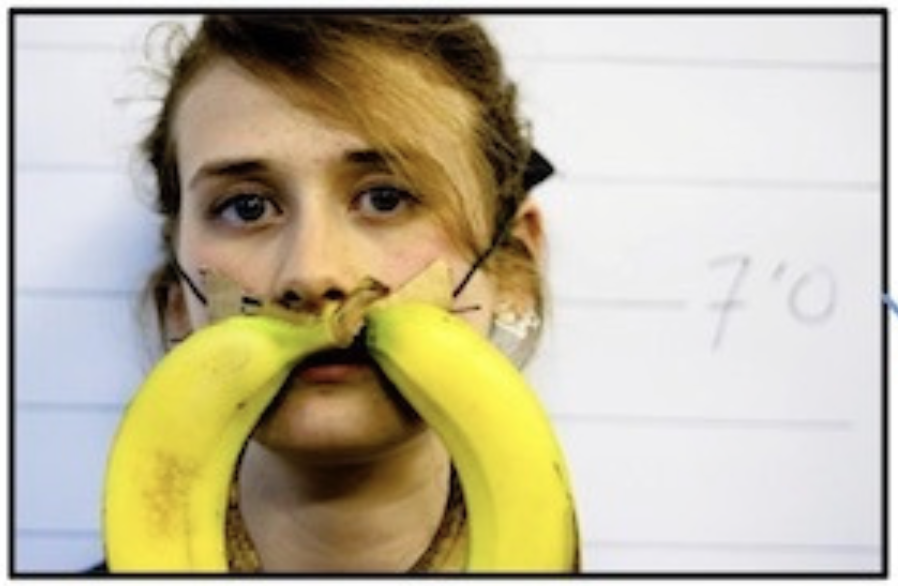
\includegraphics[width=7cm]{figures/VQAbanana}
    \caption{A Question in a Visual-Question Answering Tasks might be: {\em What is the mustache made of?}} \label{fig:vqa}  
  \end{center}
\end{figure}

\subsection{Tasks}
Let us first discuss the types of tasks that vision-language models must solve, and list some of the popular benchmark suites. For understanding, the models  can be tested on visual question answering tasks (VQA), to see if the models have acquired some  textual understanding of visual images. A related, but generative, task is that of captioning problems, where models have to generate a textual descriptions of images. Additionally, models may be tasked to do image generation. 

Let us have a look at some example tasks. For Figure~\ref{fig:vqa}, a VQA question could be: {\em What is the mustache made of?} and the system should answer: {\em Bananas}. Other typical VQA questions are to count the number of certain shapes of a certain color in a certain part of an image (to answer questions such as: {\em Is there a red block in the upper corner of the table in this scene?}). The tasks can be quite diverse, and there is a range of popular benchmarks such as MOSAIC \citep{burda2025culturally}, GLOBAL-RG \citep{bhatia2024local},  CultureVQA \citep{nayak2024benchmarking}, FoodieQA \citep{li2024foodieqa}, and MaRVL \citep{liu2021visually}. 

%Just benchmarks, or also famous models/approaches, of gaat dat te diep? Nee, dat komt later al.

\begin{figure}
  \begin{center}
    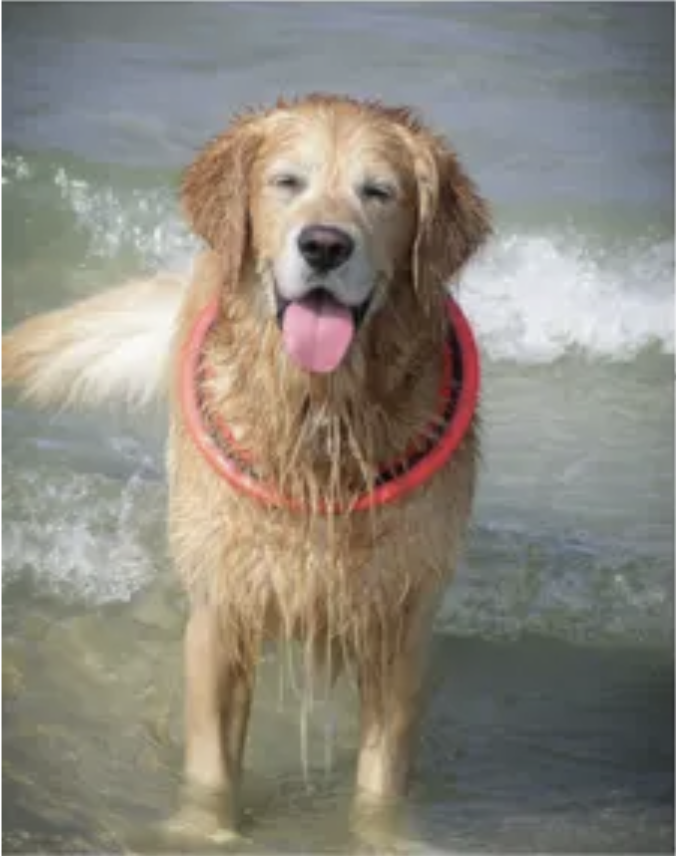
\includegraphics[width=6cm]{figures/captioning}
    \caption{A Captioning Task, possible Caption: {\em A happy dog is standing in the ocean}} \label{fig:cap}  
  \end{center}
\end{figure}



In captioning problems, a model  could be prompted to provide a caption for the scene in Figure~\ref{fig:cap}, which shows {\em a happy dog standing in the ocean}. Note that variations may be equally valid, such as {\em a wet dog}, {\em a cold dog}, or {\em a dog with a red collar standing in the ocean}. Popular benchmarks are  MS-COCO \citep{lin2014microsoft}, nocaps,\footnote{\url{https://nocaps.org}} and, for video,  MSR-VTT \citep{xu2016msr}, and VATEX  for traditional, short-caption evaluation \citep{wang2019vatex}. Newer benchmarks have been developed that focus on detailed, multi-faceted descriptions:  DetailCaps \citep{dong2024benchmarking},   VDC \citep{chai2024auroracap}, and CapArena \citep{cheng2025caparena}. %\todo{Benchmark overload. Het gaat meer om methoden uit te leggen aan de studenten dan om te laten zien dat ik de literatuur ken. Reduce the }

Typical applications of VLMs are summarization, image generation, search and retrieval, image segmentation, and object detection. The Massive Multi-discipline Multi-modal Understanding and Reasoning Benchmark (MMMU) for Expert AGI  is a comprehensive benchmark for vision-language models \citep{yue2024mmmu}. 


%!!!!!!!!!!!!!!!!!!!!!!!!!!!!!!!!!!!!!!!

%{\bf REWRITE:} Vision language models are models that can learn
%simultaneously from images and texts to tackle many tasks, from visual
%question answering to image captioning. The use cases include chatting
%about images, image recognition via instructions, visual question
%answering, document understanding, image captioning, and others. Some
%vision language models can also capture spatial properties in an
%image. These models can output bounding boxes or segmentation masks
%when prompted to detect or segment a particular subject, or they can
%localize different entities or answer questions about their relative
%or absolute positions. 

%\url{https://www.ibm.com/think/topics/vision-language-models}
%Goals: 
%- VQA (answer text questions)
%- Captioning (generate text description)
%Applications: Captioning and summarization, Image generation, Image search and retrieval, Image segmentation, Object detection, Visual question answering (VQA)

\subsection{Architecture}
Now that we have seen the types of tasks that VLMs are tested on, how could we design a model to perform these tasks? %Architectures that combine visual and language knowledge should be able to generalize, answer questions, and draw conclusions.

Language, when modeled as a sequence of tokens, is a sequential (1 dimensional) problem domain. Vision, when modeled as a  grid of pixels, is a rectangular (2 dimensional) problem domain. Correspondingly, the deep learning architectures for the two applications are different. For language, the transformer architecture is used,  finding sequential patterns, and for imaging, the convolutional neural network is used,  finding 2-dimensional patterns. It is therefore not obvious what architecture a multi-modal vision-language model should have. Indeed, it was unclear if a VLM would work at all.

Research first focused on the question if the transformer architecture would also be able to work on image processing (in addition to the conventional convolutional neural networks, CNN). Special vision transformers and tokenization schemes were  developed  that worked well in image processing \citep{dosovitskiy2020image}. 

\begin{figure}
    \centering
    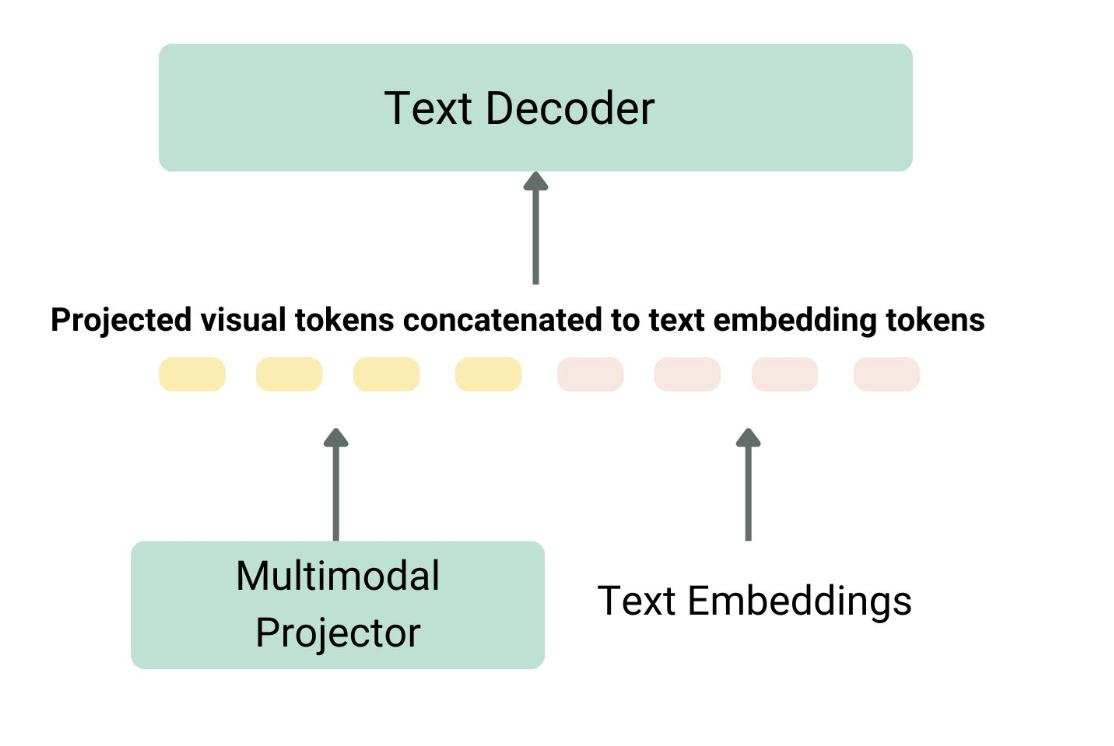
\includegraphics[width=0.5\linewidth]{figures/vlm}
    \caption{Architecture of a VLM (after LLaVa \citep{liu2023visual}, image from Huggingface) }
    \label{fig:vlm}
\end{figure}


\begin{figure}
    \centering
    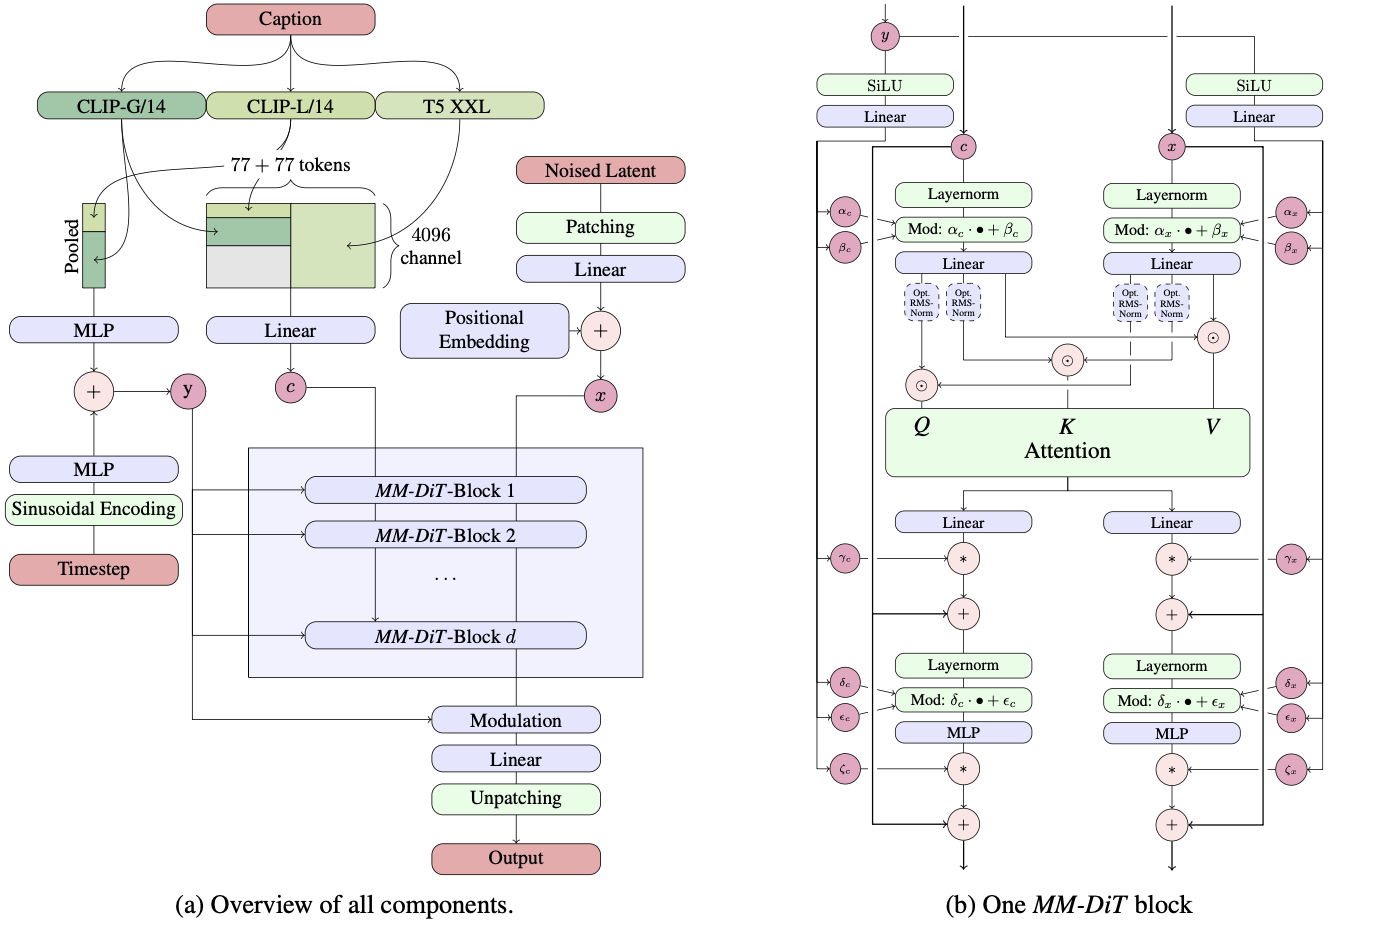
\includegraphics[width=0.95\linewidth]{figures/stable}
    \caption{Architecture of Stable Diffusion \citep{esser2024scaling} }
    \label{fig:stable}
\end{figure}

Then, an architecture was needed to combine the language and  image embeddings, and to generate language. 
In general, the architecture of a VLM consists of  an image encoder (either a CNN or a specially tokenized vision-transformer) and a text encoder that are connected to an embedding projector to align image and text representations (often a dense neural network), connecting to, finally, a text decoder (a transformer). Figure~\ref{fig:vlm} illustrates this architecture, using LLaVa as an example \citep{liu2023visual}.
The connection between the visual embedding and the textual embedding is made by a network that projects the visual embedding to another embedding, to allow unified reasoning by the model. The projector network is often a dense neural network (multi-layer perceptron, MLP). 

More elaborate architectures have been developed, and the architecture of state of the art VLMs can become quite complex, consisting of multiple transformer modules. As an example, Figure~\ref{fig:stable} shows the generative Stable Diffusion architecture \citep{esser2024scaling,weng2021diffusion,yang2023diffusion}.

\subsection{Learning Algorithm}
Now that we have seen the tasks and the architecture of VLMs, it is time to look at the type of learning algorithm that is used by the models.
The different encoders and projectors allow the VLM to be trained. The training algorithms should align and fuse the knowledge from both the visual and the language encoders. The VLM can then correlate the image and text information so that the model can analyze the query and provide an answer based on the two modalities. The literature reports a variety of  approaches for training the VLM.

OpenAI's CLIP \citep{radford2021learning}, which stands for {\em contrastive language-image pretraining}, uses contrastive learning. Contrastive learning is a form of self-supervised learning, creating supervisory signals  when there are no such labels in the dataset. The idea is to push dissimilar data points apart and pull similar data points together in an embedding space. Contrastive learning maximizes the similarity of representations for {\em positive} pairs (such as similar forms of the same image) and minimize the similarity for {\em negative} pairs (images of different objects).  %The VLM is trained on a dataset of image-text pairs. It maps the image and text embeddings from the encoders into a joint  embedding space to predict the correct pairings, it minimizes the distance between embeddings of matching pairs, and maximizes it for non-matching pairs. 

%Arch:
%- language encoder. Transformer
%- image encoder. First CNN, now ViTransformer

%Learning Algorithm:
%- constrastive. CLIP
Another approach is to use masking. Here the VLM learns to predict randomly obscured parts of an input text or image, just as it is used in language model training. The model learns to reconstruct the hidden pixels in an image given an (unmasked) caption. An example is FLAVA, or {\em foundational language and vision alignment}, which uses a vision  transformer as image encoder and  a transformer for its language encoder and multi-modal projector \citep{singh2022flava}. 

%- masking. FLAVA
\begin{figure}
    \centering
    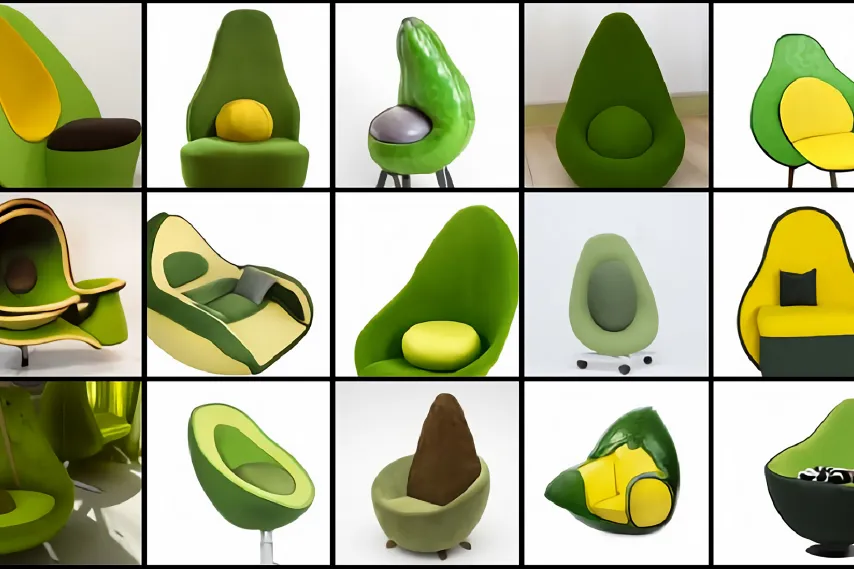
\includegraphics[width=\linewidth]{figures/dalle}
    \caption{DALL-E: Avocado Armchairs}
    \label{fig:dalle}
\end{figure}
VLM's are also used in a generative style, to generate an image based on a text prompt. Popular text-to-image models often use diffusion models \citep{ho2022large,yang2023diffusion}. Well-known examples are Google’s Imagen \citep{baldridge2024imagen}, Midjourney, OpenAI’s DALL-E \citep{betker2023improving} and Stability AI’s stable diffusion \citep{esser2024scaling}. DALL-E 2 uses a diffusion model conditioned on CLIP image embeddings. Figure~\ref{fig:dalle} shows DALL-E's well-known surrealistic avocado armchairs.  

%- pretrained. LLAVA

%Contrastive: maps the image and text embeddings from both encoders into a joint or shared embedding space. The VLM is trained on datasets of image-text pairs and learns to minimize the distance between embeddings of matching pairs and maximize it for nonmatching pairs. CLIP

%Masked: in masked image modeling, VLMs learn to reconstruct the hidden pixels in an image given an unmasked caption. The multimodal encoder applies a cross-attention mechanism to integrate textual and visual information. FLAVA’s training encompasses masked modeling along with contrastive learning.

%Generative: 
%learning to generate new data. Text-to-image generation produces images from the input text, while image-to-text generation produces text—such as captions, image descriptions or summaries—from an input image. Examples of popular text-to-image models include diffusion models, such as Google’s Imagen, Midjourney, OpenAI’s DALL-E (beginning with DALL-E 2) and Stability AI’s Stable Diffusion.

%Pretrained:
Pretraining vision language models from scratch is expensive, and since a VLM consists of a language model and a vision model, we could try to see if it is possible to build a VLM out of one or two existing models, that have already been pretrained before.
Both a pretrained LLM and a pretrained vision encoder can be used, to which a mapping network can be added that projects the visual embedding to the textual input space of the language model.
An example is LLaVA, which stands for {\em large language and vision assistant}.  LLaVa uses the Vicuna language decoder and the CLIP ViT visual encoder, and their outputs are merged into a shared dimensional space using a linear projector \citep{liu2023visual}.

Many vision language models have been developed. VLMs tend to perform well on benchmark tasks and they are often used for decision making in agents. 
VLMs have become so popular that many current open and commercial LLMs are  VLMs: DeepSeek-VL2, Gemini 2.0 Flash, GPT-4o, Llama 3.2, NVLM, Qwen 2.5-VL.



\begin{figure}
    \centering
    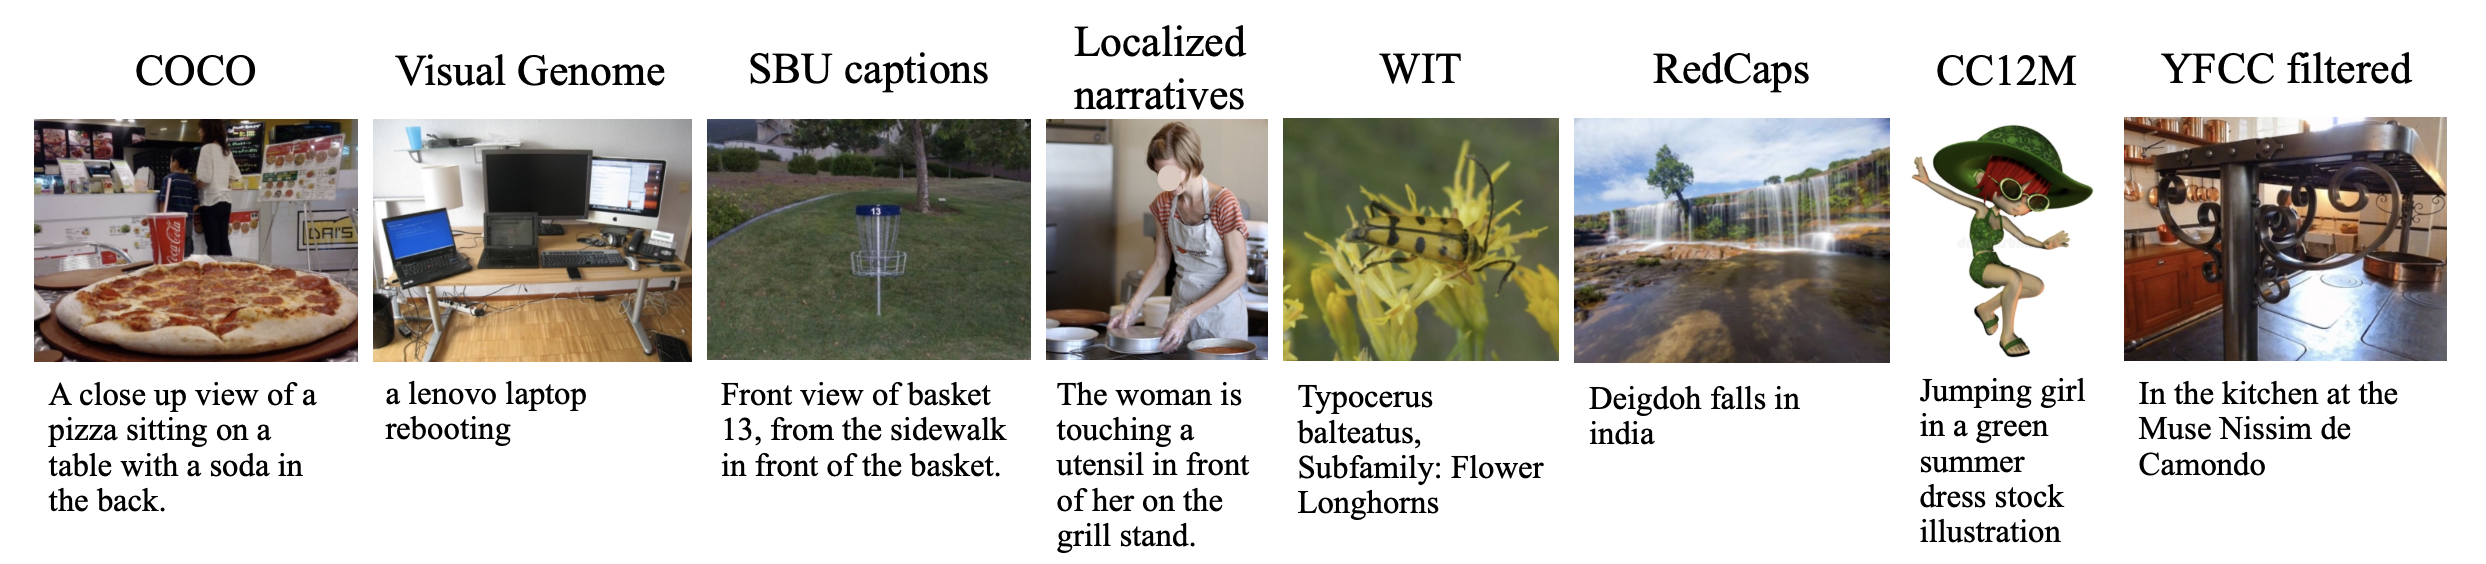
\includegraphics[width=\linewidth]{figures/flava}
    \caption{Flava Pretraining Image-Text Dataset Examples \citep{singh2022flava}}
    \label{fig:flava}
\end{figure}

\subsection{Results}
Let us take a look at how well VLMs perform at captioning and image generation by looking at some of the examples that are reported in the literature.

Vision language models have produced imaginative and inspiring results ranging from visual question answering, object detection, image captioning to text-to-image generation. An example of the test dataset that is used in Flava is shown in Figure~\ref{fig:flava}.  The successor of DALL-E 2, DALL-E 3, focused on training on highly descriptive generated image captions, yielding even more impressive results \citep{betker2023improving}. Some of the prompt following image generation capabilities of DALL-E 3 are shown in Figure~\ref{fig:dalle3}. Figure~\ref{fig:stablediff} shows examples from stable diffusion (based on the  rectified-flow diffusion models). 


\begin{figure}
    \centering
    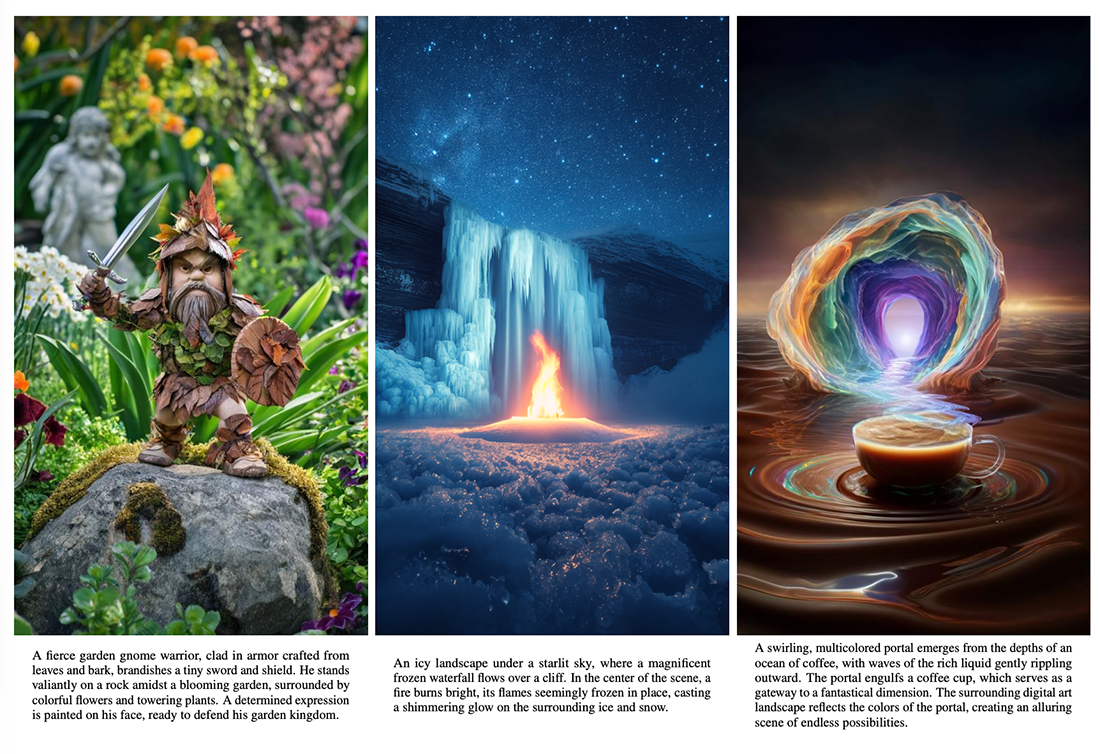
\includegraphics[width=\linewidth]{figures/dalle3}
    \caption{Prompt Following Text-to-Image Examples from DALL-E 3 \citep{betker2023improving}}
    \label{fig:dalle3}
\end{figure}


\begin{figure}
    \centering
    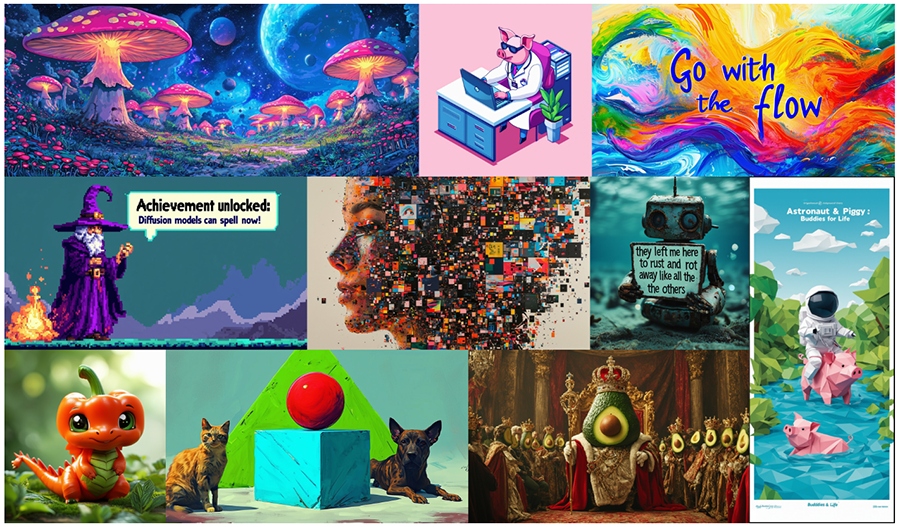
\includegraphics[width=\linewidth]{figures/stablediff}
    \caption{Stable Diffusion Examples \citep{esser2024scaling}}
    \label{fig:stablediff}
\end{figure}


\begin{figure}
    \centering
    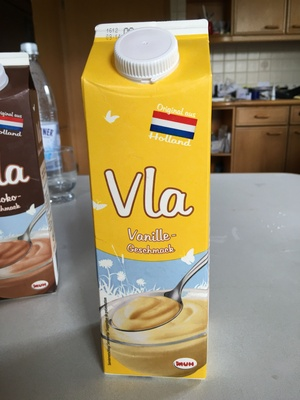
\includegraphics[width=0.4\linewidth]{figures/vla.jpg}\ 
        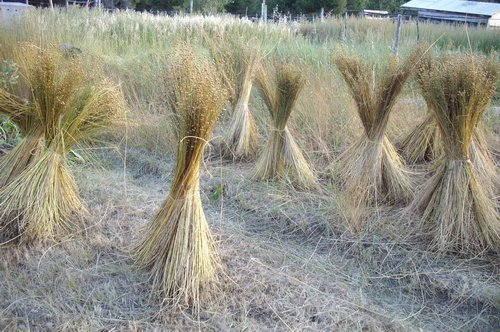
\includegraphics[width=0.4\linewidth]{figures/vlas.jpg}
    \caption{VLA has a different meaning in different languages. So has Vlas. (A hint of which language this is flagged in one of the pictures)}
    \label{fig:vla}
\end{figure}

\section{Decisions \& Vision Language Action Models}\label{sec:vla}

%\paragraph{Vision-Language-Action Models}
To act, agents must make decisions, and to make decisions, different options must be weighed. %The previous chapter showed methods for external prompt optimizers to search the tree of possibilities and in-context learning. We also saw in Section~\ref{sec:decisions} that the transformer architecture can  be pretrained to facilitate decision making, and reinforcement learning. %At the end of this chapter we will discuss this approach in more depth. %\todo{AGAIN??? We did that in 6.2.4. Hmm. In this chapter the DT story is longer. Where does it fit best? It does fit in 6.2.4. But also in 7.4. Gewoon zeggen dat we het al eens eerder gezien hebben?}
As we will see in this section, %in addition to training transformers on sequences of tokens that represent language and pixels, 
we can  train transformers on episodes of states, actions and rewards $\{(s,a,r)\}$ (see also Section~\ref{sec:decisions}).
%
These models are trained on sequences of language, vision, and robotic actions. Vision-language-action models, VLAs, (Figure~\ref{fig:vla}) are trained to output robot API commands, which are a special type of language: the language of commands to steer robotic movement. %Various pretraining and interacting on large datasources has yielded impressive generalization by VLAs \citep{black2024pi_0,team2023gemini}.

%After vision, the next step is to add actions to the model. Models that are trained on vision, language and actions are called vision-language-action models, or VLA (see Figure~\ref{fig:vla}). 
The task of a VLA is  to understand a visual scene, and, when given a textual command, instruct a robot arm to perform an appropriate action, depending on what the model sees through the camera.
These models have shown impressive results of robots generalizing to unseen situations, successfully performing tasks.

\begin{figure}
    \centering
    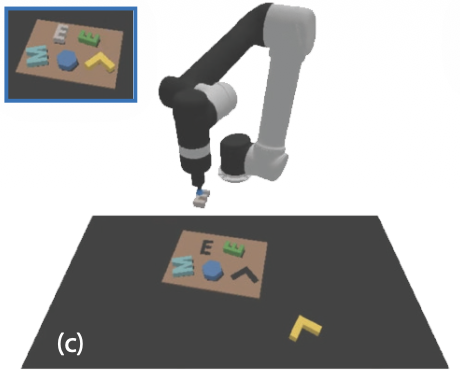
\includegraphics[width=0.5\linewidth]{figures/cliport1}
    \caption{Example from CLIPort: {\em put the gray letter E in the left letter E shape hole} \citep{shridhar2022cliport}}
    \label{fig:cliport1}
\end{figure}

\subsection{Tasks}
The main task of VLAs is to perform instructions in the real world, and to do so in a general way, in a changing environment. When a robotic manipulation model has been trained to pick up a set of red pencils, and the task changes to pick up blue pencils, then it would be nice if the model generalizes, and we do not have to assemble a new training set involving blue pencils and re-train the model again from scratch. We also want our  model to recognize objects, and recognize when an object is oriented differently,  has moved, or the lighting changes. The model should know how to use a robot arm to manipulate objects, and how to perform different actions. See Figure~\ref{fig:cliport1} for an example, taken from the CLIPort paper \citep{shridhar2022cliport}.


\begin{figure}
    \centering
    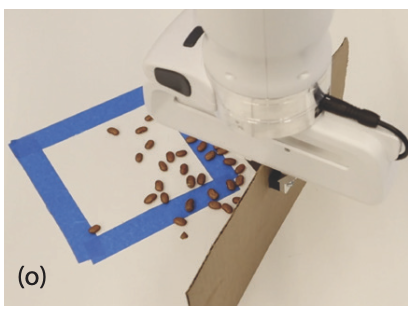
\includegraphics[width=0.5\linewidth]{figures/cliport2}
    \caption{Another Example from CLIPort: {\em sweep the beans into the blue zone} \citep{shridhar2020alfworld}}
    \label{fig:cliport2}
\end{figure}

The hardest task for VLAs is to combine these scenes, objects and  actions to manipulations that are complicated combinations of what the model has seen during training, and to generalize to unseen combinations. Especially long-horizon navigation through complex, changing, environments (perhaps even outdoors) is a complex challenge \citep{shridhar2022cliport}.

In realistic human-robot interaction settings,
collecting additional demonstrations is often infeasible.
To perform  high-level tasks, such as in Figure~\ref{fig:cliport2}, the VLA must be able to recognize objects, their poses, and segmentations of instances. The model must also be able to understand language, and relate the meaning of language to the meaning of visual objects and to the meaning of robotic actions.

As we will see, language provides an intuitive interface for specifying goals and  for  transferring semantic concepts across tasks. Furthermore, the work on VLMs has shown how to semantically connect different kinds of embeddings.

%Describe
%significantly improved generalization to novel objects, the ability
%to interpret commands not present in the robot training data (such as placing an object onto a particular
%number or icon), and the ability to perform rudimentary reasoning in response to user commands (such
%as picking up the smallest or largest object, or the one closest to another object). We further show that
%incorporating chain of thought reasoning allows RT-2 to perform multi-stage semantic reasoning, for
%example figuring out which object to pick up for use as an improvised hammer (a rock), or which type
%of drink is best suited for someone who is tired (an energy drink).

%long-horizon navigation through complex, outdoor envi-
%ronments from natural language instructions

%capable of solving a variety of language-specified tabletop tasks from packing
%unseen objects to folding cloths, all without any explicit representations of object
%poses, instance segmentations, memory, symbolic states, or syntactic structures.
%Experiments in simulated and real-world settings show that our approach is data
%efficient in few-shot settings and generalizes effectively to seen and unseen se-
%mantic concepts. We even learn one multi-task policy for 10 simulated and 9
%real-world tasks that is better or comparable to single-task policies.

%Mobility VLA in a 836m2 real world environment and
%show that Mobility VLA has a high end-to-end success rates on previously unsolved
%multimodal instructions such as “Where should I return this?” while holding a plastic
%bin.



%Generalization: Give textual instruction to robot to move in visual scene. 

\subsection{Architecture}
Now that we have seen the task and the challenges, let us look at possible model architectures. Again, they can become quite complex.
The transformer architecture is well suited to learn patterns in sequential data, as the  results on natural language show.  Intuitively, this suggests that transformers may also work well to model sequential decision problems, the type of problems that are often solved in reinforcement learning for robotic action, as we discussed in Section~\ref{sec:sdp} (and further in depth in Section~\ref{sec:icrl}). These problems consist of a state, from which actions cause the system to enter a new state, which has actions, etc. The transformer architecture is well suited to model these problems.

Early work on decision transformer (DT) \citep{chen2021decision,janner2021offline} showed that on offline (static) reinforcement learning  problems, the GPT architecture was indeed able to learn optimal policies.   The decision-pretrained  transformer (DPT) \citet{lee2023supervised,wang2024transformers} showed that the basic transformer architectures can  be pretrained and finetuned on decision  traces.  Section~\ref{sec:decisions} discusses decision traces further.  

Following pioneering work on CLIPort \citep{shridhar2022cliport,shridhar2020alfworld}, VLAs are often built on VLMs, where the robotic commands are used as regular language tokens. Let us have a closer look at some representative models.


The goal of  Mobility VLA \citep{chiang2024mobility} is navigation. This VLA is created by combining  a long context VLM with topological maps, as illustrated in Figure~\ref{fig:mobility}.
\begin{figure}
    \centering
    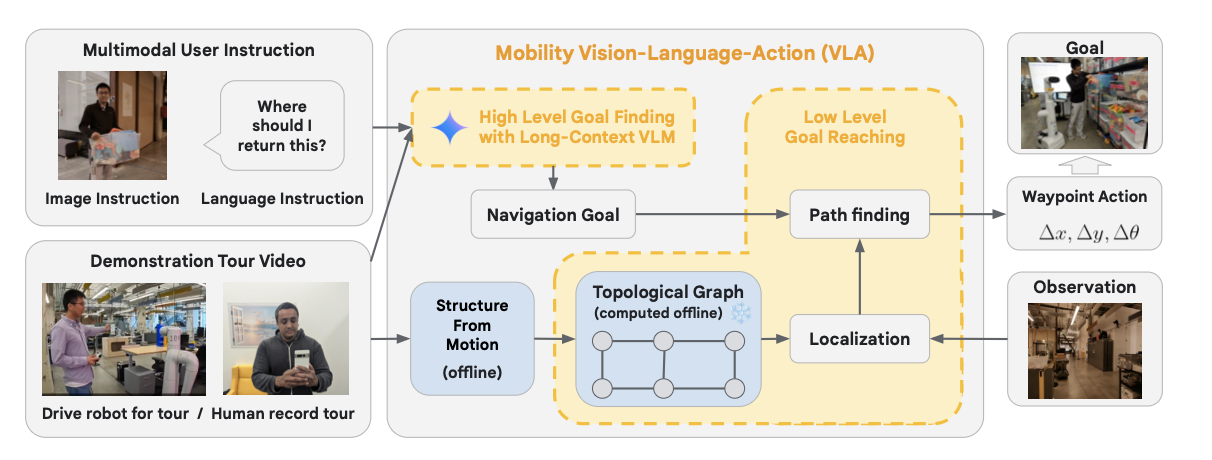
\includegraphics[width=0.95\linewidth]{figures/mobility}
    \caption{Mobility VLA Architecture: Long Context VLM and Topological Maps \citep{chiang2024mobility}}
    \label{fig:mobility}
\end{figure}
Mobility VLA is used on a problem category of navigation tasks called {\em multi-modal instruction navigation with demonstration tours} (MINT). In this dataset, an environment prior is provided through a previously recorded demonstration
video. The model consists of a two-level  VLA that combines the environment
understanding and common sense reasoning  of long-context VLMs with a 
low-level navigation policy based on topological graphs. The high-level policy is created by combining  user instructions from a long-context VLM that finds the goal frame in a demonstration  video. Then, a low-level policy starts at this  goal frame to traverse a topological graph to generate the robot action instructions at every timestep.

LM-Nav \citep{shah2023lm} uses a different architecture, based on existing models. It takes as input a set of raw observations
from the target environment and from free-form textual instructions. From this, it derives an action plan using three pretrained models: a  language model (LLM) for extracting landmarks, a vision-language model (VLM)
for grounding, and a visual-navigation model (VNM) for execution (not unlike the topological map previously discussed). Together, these models  enable LM-Nav to follow textual
instructions  from visual observations  without any finetuning. Figure~\ref{fig:lmnav} shows an illustration of the approach.
\begin{figure}
    \centering
    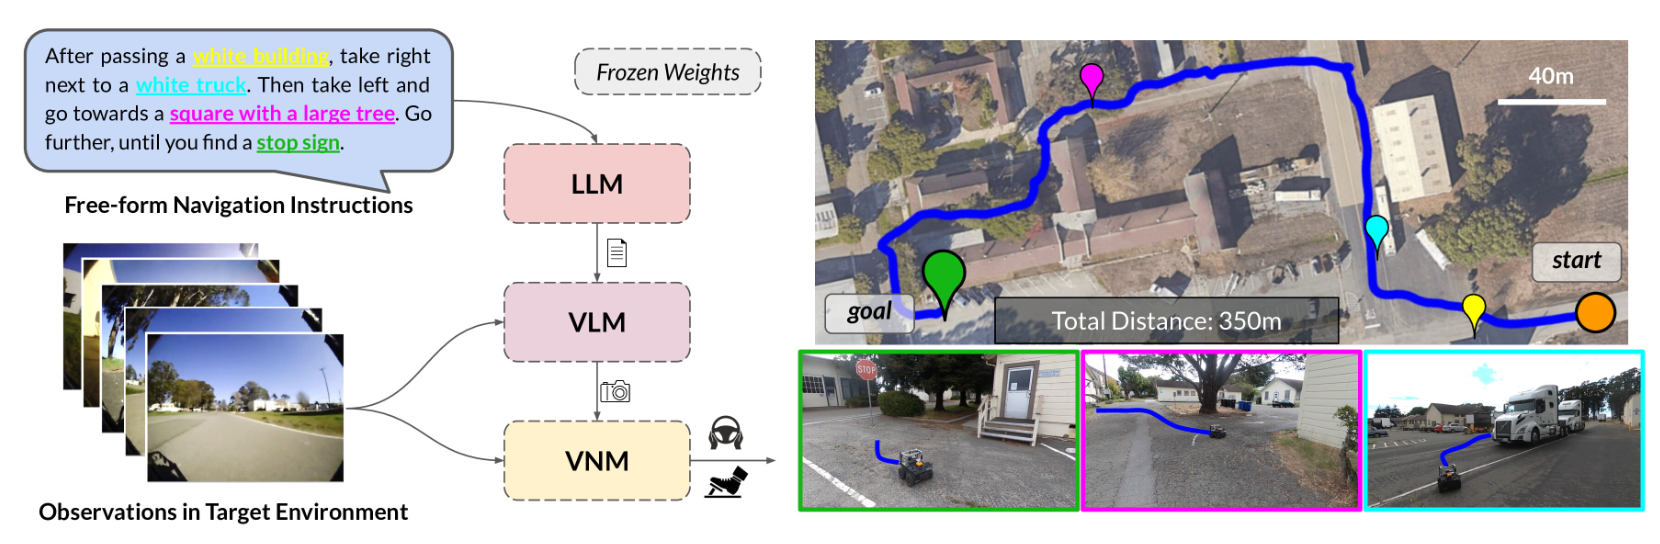
\includegraphics[width=0.95\linewidth]{figures/lmnav}
    \caption{Three-LLM Architecture of LM-Nav \citep{shah2023lm} }
    \label{fig:lmnav}
\end{figure}


Google's RT-2 \citep{brohan2023rt} uses a different approach. The idea of RT-2 is to leverage knowledge from the web to inform robotic control: the robot should learn how to act from watching videos. A standard vision language model is finetuned both on textual robotic trajectory data and on
Internet-scale vision-language tasks, such as visual question answering. Robotic  actions are expressed as regular text tokens and are incorporated 
directly into the training set in the same way as natural language tokens, as shown in Figure~\ref{fig:rt2}.
\begin{figure}
    \centering
    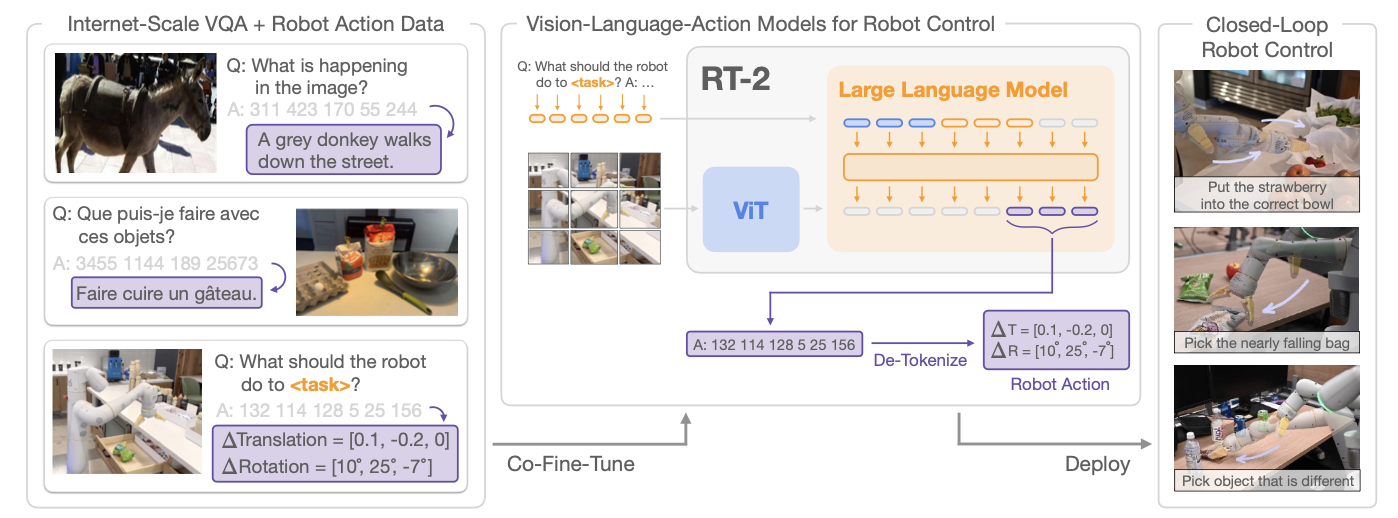
\includegraphics[width=0.95\linewidth]{figures/rt2}
    \caption{RT-2 Architecture:  VLM trained using Robotic Actions as Text Tokens \citep{brohan2023rt}}
    \label{fig:rt2}
\end{figure}
A similar approach is taken by Magma \citep{yang2025magma}. Magma is pretrained on  heterogeneous datasets spanning from images and videos to robotics data. However, in Magma the actionable visual objects  in images
are labeled by special tokens (Set-of-Mark) for action grounding. Similarly, object movements (such as the trace of human hands or
robotic arms) are labeled by Trace-of-Mark 
to ease action planning. Figure~\ref{fig:magma} provides an illustration.
\begin{figure}
    \centering
    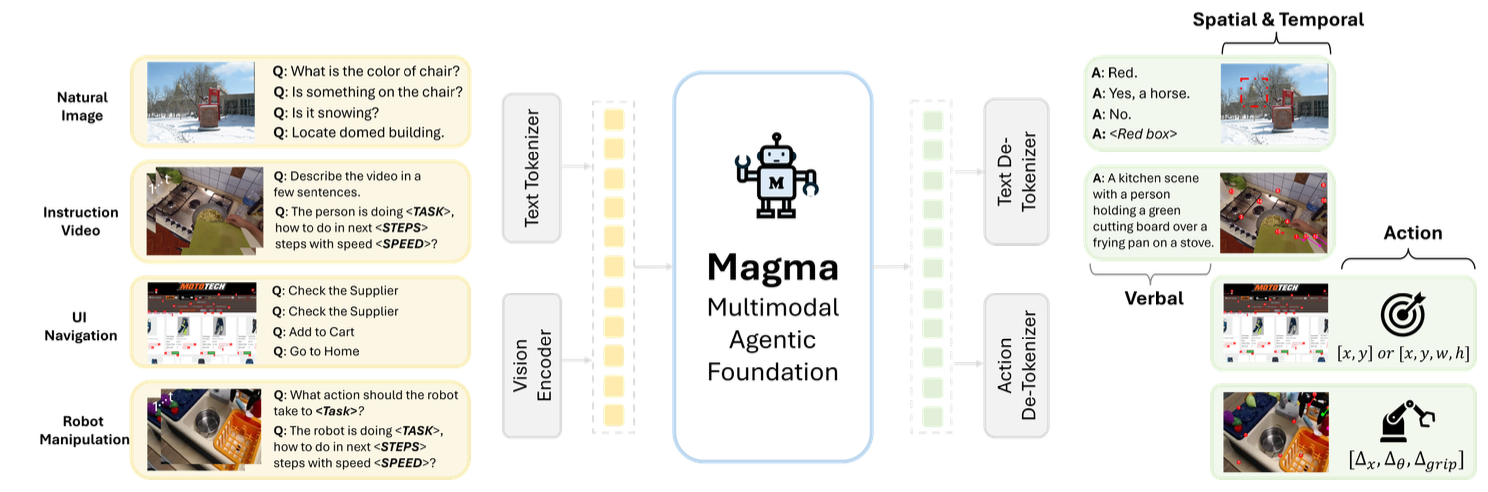
\includegraphics[width=0.95\linewidth]{figures/magma}
    \caption{Magma Pretraining Pipeline \citep{yang2025magma}}
    \label{fig:magma}
\end{figure}

Finally, a VLA called $\pi_0$ \citep{black2024pi_0} stresses the reinforcement learning approach by using a pretrained late-fusion vision-language model, as well as a diverse cross-embodiment dataset with a variety of  manipulation tasks. The model is inspired by the Transfusion approach \citep{zhou2024transfusion}. This model is adapted to robot control by adding a separate
action expert that produces actions via flow matching, for fluent manipulation skills. The resulting model
can either be used directly to perform tasks based on a prompt, or be further finetuned on higher-quality data to enable complex multi-stage
tasks, such as folding multiple articles of laundry or assembling a box (see Figure~\ref{fig:pizero}).  
\begin{figure}
    \centering
    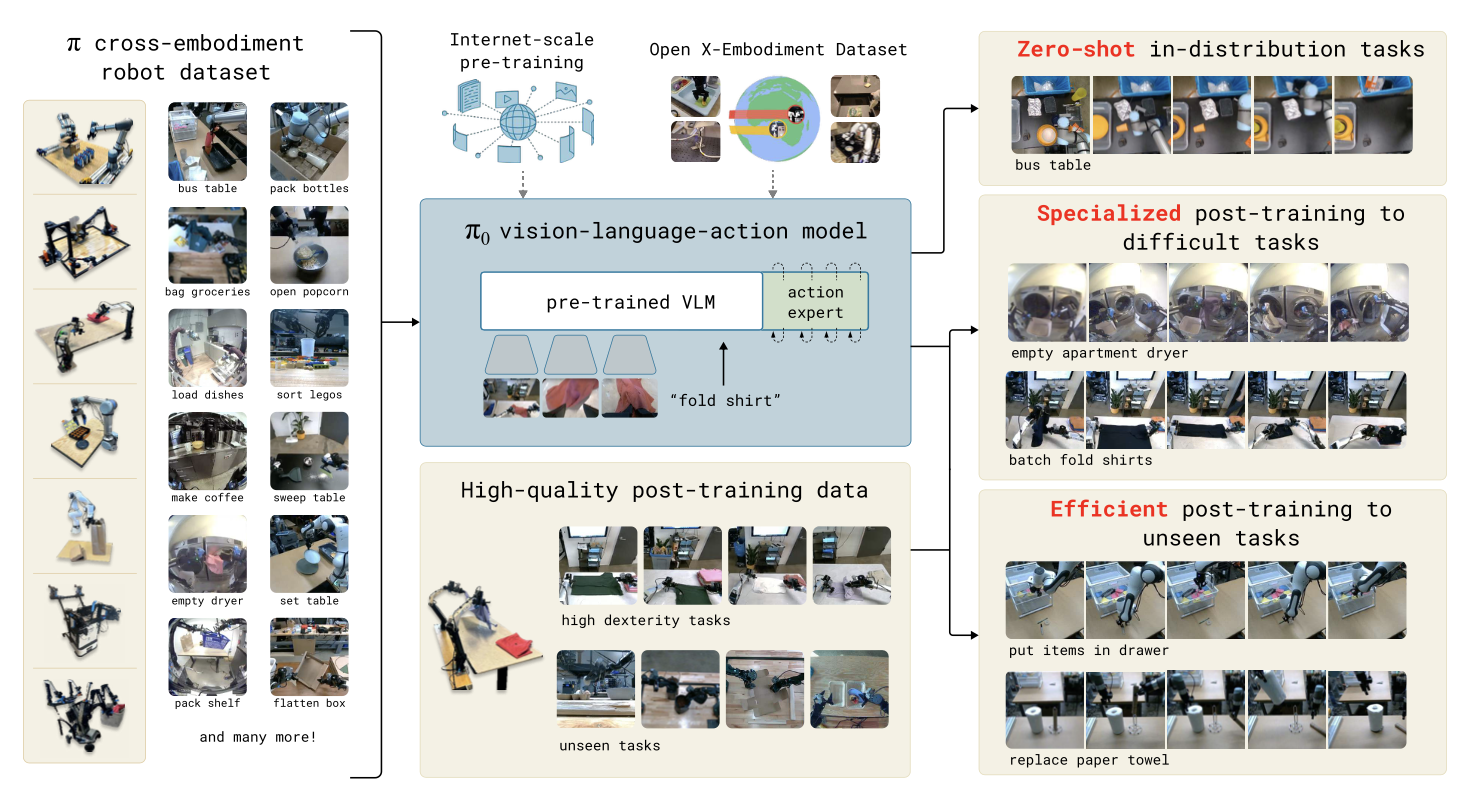
\includegraphics[width=0.95\linewidth]{figures/pizero}
    \caption{Architecture of $\pi_0$. The model is based on a VLM, enhanced with a cross-embodiment dataset \citep{black2024pi_0}}
    \label{fig:pizero}
\end{figure}









\subsection{Learning Algorithm}
The model architecture of most VLAs is based on VLMs, in some cases augmented with navigation map data. The  robotic action commands are typically encoded as regular text commands. Likewise, for pretraining and finetuning typical LLM self-supervised learning algorithms are used, similar to VLMs and decision transformers. Sometimes existing pretrained models are used, to reduce the training expense.


\subsection{Results}
Various VLA models have been
created that achieve impressive zero-shot results, generalizing behavior to unseen situations. 
\citet{chiang2024mobility,brohan2023rt,yang2025magma} are examples of
VLA models for robotic action, achieving complex tasks such as navigation, table top manipulation, or even folding laundry \citep{black2024pi_0}. 


VLAs have shown impressive and imaginative results, where robots were able to generalize at inference time without the need for retraining. A survey of VLAs can be found in
\citep{ma2024survey}.

The results are best appreciated from seeing a video.
For $\pi_0$, a video is  available.\footnote{\url{https://www.physicalintelligence.company/blog/pi0}} 
For RT-2,  a video is also  available.\footnote{\url{https://robotics-transformer2.github.io}} 




%Embodied problems require an agent to understand  semantic aspects of the world: the topology, the repertoire of skills available, how these skills influence the world, and how changes to the world map back to language. When the model is prompted to move a cup on a table, it helps when the LLM knows if the agent has limbs that allow it to move objects, and whether it is in a room where a table and a cup are present.

%By leveraging environment feedback, LLMs are able to form an inner monologue that allows them to more richly process and plan in robotic control scenarios.
%
%Language models contain a large amount of information about the real world \citep{ahn2022can}. In theory, this may allow the model to exhibit realistic reasoning about robotic behavior. %However, the models do not have knowledge about particular embodied aspects of a particular robot. 
%If we could compare a list of intermediate reasoning steps with a list of possible movements of the robot in its environment, then we could prevent the model from suggesting impossible joint movements and actions, and prevent errors or accidents. 
%Such an approach has been tried in the Say Can paper
%\citep{ahn2022can}. Say Can learns a value function \citep{kaelbling1996reinforcement} of the behavior of a robot in an environment using  temporal difference reinforcement learning \citep{sutton1988learning}. This value function is then  combined with prompt-based reasoning by the language model, to constrain it from suggesting impossible or harmful actions. 
%
% {\bf What does SayCan say? Is it like Scratchpad?}
% Note that Scratchpad was trained by supervised learning on a
% pre-existing dataset. The goal of Say-Can is to create  a robotic
% affordance model, by using reinforcement to learn a value
% function. A separate language model is used for  prompt learning, to
% incorporate the learned value function in the prompts.  
%
%The goal of Say Can is to ground the language model in robotic
%affordances. %  The affordance model is learned interactively by reinforcement
% learning, and then applied using prompt-based learning by
% the LLM. 
% The robot can act as the language model’s hands and eyes, while
% the language model has high-level semantic knowledge about the
% task.  The LLM (Say) provides a task-grounding to find the actions to
% achieve the high-level goal. The learned affordance function (Can)
% provides a world-grounding to allow what is possible. 
% Reinforcement
% learning learns language-conditioned value functions that provide affordances of what
% is possible in the world.
%Say Can is evaluated  on 101
%real-world robotic tasks, such as how to solve tasks in a kitchen environment (see Figure~\ref{fig:saycan}).


%\begin{figure}
%  \begin{center}
%    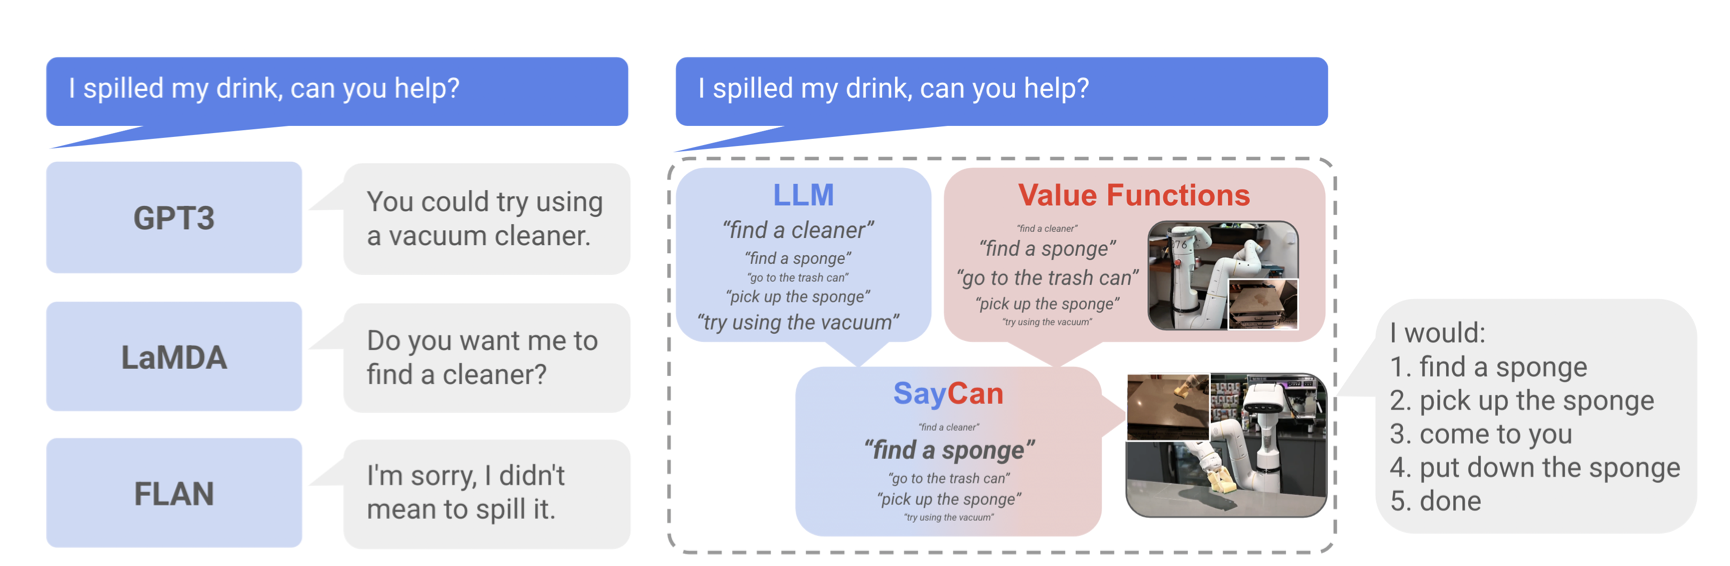
\includegraphics[width=14cm]{figures/saycan}
%    \caption{Say Can compared to other language models \citep{ahn2022can}}\label{fig:saycan}
%  \end{center}
%\end{figure}






%\citet{liu2023llm} combine an LLM with  a
%combination of teleoperation and Dynamic Movement Primitives is
%employed for action correction.


\section{World Models, Physics, and Planning}\label{sec:world}

%\paragraph{World Models}
To a VLM, an image consists of pixels without a deeper intrinsic meaning. However, agents that interact with the world need knowledge about physical aspects of that world. %As we discuss in Section~\ref{sec:world}, 
The models need an understanding of what is physically possible, so that agents do not walk through walls, as they still sometimes do in video games. 
%As LLMs incorporate more data modalities, they acquire more world knowledge. The multi-modal models that we discuss in this chapter increasingly fit the requirements to act as a source of knowledge about the world in which agentic LLMs operate. 

%Agents receive feedback when they act in the world. A world model requires a mechanism to learn from this feedback. Reinforcement learning, the type of machine learning that learns actions from feedback, offers such a mechanism.
%World models have been researched for quite some time in machine learning. In model-based reinforcement learning in particular, world models play a central role \citep{sutton1991dyna,moerland2023model,hafner2020mastering,plaat2020deep}.
%, and the training of world models has been studied. 
%These world models are trained on feedback from interaction of the agent with the world. %A model is built that  is then used to improve further interactions by the agent with that world. 
%Reinforcement learning provides a useful framework for training world models, and reinforcement learning methods are used extensively to build agentic world models with a form of understanding of physics. 

%\paragraph{Decision Transformer}
%\todo{Hmm. Is dit nu ge-delete?}


%The new modalities introduce new names: vision-language models are called VLMs, models with robotic actions are called VLAs, and models that aim to understand the physics of the world  are called {\em world models}. Note that from now on we may use the term {\em LLM} to include these new, richer models. 
%We will now start with the first modality that is added to LLMs: vision.

%In this section we will introduce world models. 
World models help agents understand the world, allowing them to act effectively in the physical world, taking actions that make sense. Originally, LLMs are language models. We can converse with them in natural language, and they necessarily contain some knowledge of the world, but they were not specifically trained to have a wide and deep understanding of worldly affairs. Some researchers argue that in order for agentic LLMs to be truly successful, and for LLMs to reach a high level of general intelligence, research into world models should be strengthened \citep{sutton2022alberta,matsuo2022deep,lecun2022path,klindt2026does}.

%Vision language models add an important skill, allowing visual understanding by the agent, and VLAs add certain types of actions to the model, mostly in the realm of robotic arm movement. Research into world models extends this trend, and specifically focuses on adding knowledge to the reasoning model that will allow our agents to function well in the physical world. If this sounds as if the field is in motion, it is. World models are an active field of research, and we will discuss as much as we can of the state of the art. 


%LLMs are more and more regarded as world models from which an agent can sample to learn to improve a policy of good actions. Therefore, in this section we will review recent world model research. 

Agents and robots that act in the world need a rudimentary understanding of the physics of the world.
One of the challenges for training an LLM is to ground its understanding of the physical world and of the possible robotic actions into reality.
One way to do this is to learn an agentic model of the world (environment) from feedback on actions.

%From VLM, to VLA, the step to training a World model seems a small next step. 
The term {\em world model} has been used in AI in other contexts. Most notably, it refers to the {\em model} in model-based reinforcement learning \citep{ha2018world,moerland2023model,sutton1991dyna} (see next section). %The meaning of the term {\em world} in reinforcement learning is the same as in agentic LLM: 
This model contains a local copy of some knowledge of the environment, based on the interactions it has had with the environment, to be used to improve the action policy. 
The world model contains an efficient, compressed, learned representation of the world \citep{hafner2018learning,plaat2020deep}. The representation of a world model is often called an abstract or  {\em latent} representation, to contrast it with the regular representation of the real world in the environment. 
World models are often trained to contain knowledge about  physics and certain spatial properties, that puts restrictions on the agent's actions. % (to prevent it from attempting to walk through walls, for example).  
The precise contents of the world model depends on the domain in which the agent operates. 




Note that in a just few chapters we have progressed from  understanding language to understanding the world. The goal of a large {\em language} model is to understand some semantics of natural language from statistical patterns in text, to be used for question answering and translation. The goal of a {\em world} model  is to understand causal relations in the laws of physics, to be used to simulate future world states for our agent. Quite some new technology is necessary to go from LLM to agentic LLM. 


We start with a look at how world models are currently used in agentic LLM.

\subsection{Tasks}
World models should encapsulate knowledge of the world, so that an agent can perform meaningful actions. The actions should be grounded in the physical world. For example, the model should understand the limitations of the joints of a robot arm that it is commanding; a navigational agent should understand some physics, such as the concept of gravity, of distance, and that walls are solid objects; a financial agent should understand the consequences of a negative bank balance. Often this is the type of information that humans take for granted, and we are surprised when an agent fails to understand such basic things about the world in which it operates. VLMs that are only trained on pixels may miss the semantic meaning of a specific texture, whether it is a garment, smoke,  or a wall. 

Standard pretrained LLMs already contain some useful world knowledge. They learn acceptable textual behavior using reinforcement learning with human feedback (RLHF), and acceptable mathematical and coding behavior using reinforcement learning with verifiable rewards (RLVR). Some early approaches use LLMs as pretrained world model without any finetuning. 
A natural way to learn about the physics of the world is  through interaction: agents can learn acceptable physical behavior through a reinforcement learning-style reward function.

%Reasoning via Planning (RAP) \citep{hao2023reasoning}, for example, follows a reinforcement learning design where the LLM is used for the separate functions of an MDP (action selection function, transition function, reward function), with a Monte Carlo Tree Search  planner (MCTS)~\citep{browne2012survey}. RAP achieves good results in blocksworld and GSM8K, using GPT and LLaMa LLMs in a pure ICRL setup, with MCTS. 

%Later approaches pretrain and finetune LLMs specifically as world model.
The goal of world models in model-based reinforcement learning is to improve the sample efficiency of learning from interaction, by planning with the world {\em model} instead of sampling from the {\em real} world. This is especially useful when interacting with the world is more expensive than performing a simulation, as will often be the case in agentic LLM. In the approaches that we will discuss, LLM world models  use methods from model-based reinforcement learning (see Section~\ref{sec:mbrl}). Currently, world model approaches in LLM are  quite diverse. To show which tasks world models are used for in LLMs, we will discuss three examples: WorldGPT, WebDreamer, and WorldCoder. 

\paragraph{WorldGPT}
The goal of 
WorldGPT \citep{ge2024worldgpt} is to solve visual question answering and embodied planning tasks, including audio-video question answering. WorldGPT learns a world-VLM from videos.
It uses a  latent space VLM with external knowledge bases and long-term memory. 

\paragraph{WebDreamer}
The goal of WebDreamer \citep{gu2024your} is to improve efficient learning of Web-interaction tasks, such as e-commerce. WebDreamer enables web-agents to simulate actions before execution, and thus be faster and more sample efficient (by not having to act in the real web to gather experience). WebDreamer is a model-based reinforcement learning approach in a web-world. (The name is derived from {\em Dreamer}, a series of influential model-based reinforcement learning latent dynamics models~\citep{hafner2018learning,hafner2019dream,hafner2023mastering}.) Typical tasks are to find products on e-commerce sites. It does so by training a small model from a large model, allowing efficient simulation.

%Be able to use LLM to simulate. Enable Model-based Planning for Web Agents before committing to real action. How can we build effective world models for the Internet? Unlike traditional world models in RL focusing on improving data efficiency in the agent learning process, LLM-based world models emphasize decision-making over simulation fidelity, leveraging broad world knowledge for planning. 

\begin{figure}
  \centering
    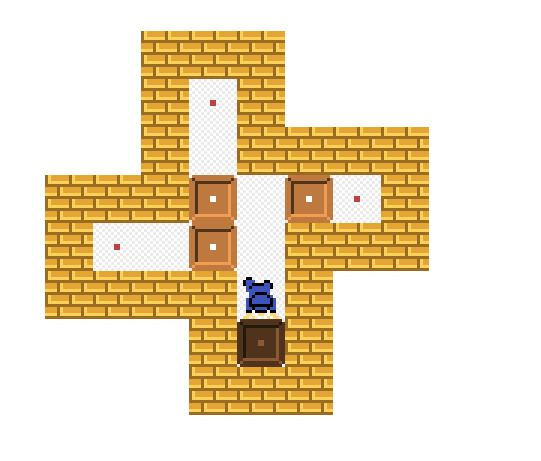
\includegraphics[width=7cm]{figures/sokoban}
    \caption{Sokoban for WorldCoder~\citep{tang2024worldcoder}}\label{fig:sokoban}
\end{figure}

\begin{figure}
  \centering
    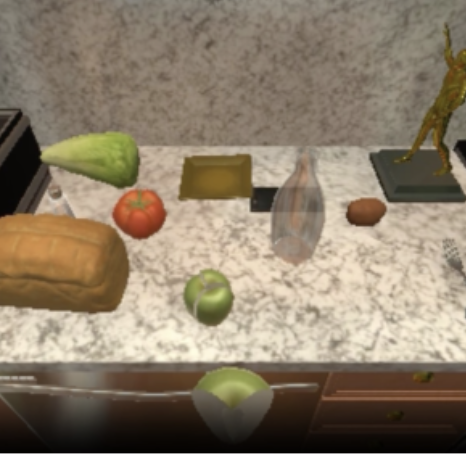
\includegraphics[width=6cm]{figures/alfworld}
    \caption{AlfWorld for WorldCoder \citep{tang2024worldcoder}}\label{fig:alfworld}
\end{figure}

\paragraph{WorldCoder}
The goal of WorldCoder \citep{tang2024worldcoder} is  also to improve sample efficiency, but the approach is different. %Its goal is also to improve sample efficiency, but i
WorldCoder improves efficiency by generating the dynamics model (transition function and reward function) in interpretable Python code, which is then used in a standard model-based reinforcement learning design. The generated Python code executes more efficiently than LLM inference does. WorldCoder is used in grid-tasks (Sokoban, see Figure~\ref{fig:sokoban}) and domestic task planning (AlfWorld, see Figure~\ref{fig:alfworld}).


\subsection{Architecture}
The purpose of a world model is to add semantic meaning to  observations---actions having consequences---something that LLMs and VLMs may struggle with. When does a pixel belong to a floor to walk on (restrict $y$ movement) and when is it part of  a wall to stop you (restrict $x$ movement)?  A reward function  provides feedback information on which actions are good, and which are not. Thus, world model architectures often use a reinforcement learning setting, in which an action policy is trained from feedback rewards. We can think of a world model as a VLM with a policy learner inside. 

WorldGPT,  WebDreamer, and WorldCoder use different  architectures for their world model, which we will now discuss in more detail. 

\begin{comment}
\paragraph{WorldGPT Summary}
\begin{itemize}
    \item Goal: Understand World Dynamics. WorldGPT is capable of synthesizing dynamic scenes that change according to complex interactions.
    \item Data: Analyze internet videos.
    \item Architecture: WorldGPT is World Simulator. Help synthesize multimodal instruction instances. Built on MLLM. Specialized/long-term tasks: cognitive architecture (memory, knowledge retrieval, context reflection). Composed of 3 modules: Multimodal encoders, LLM to predict state transisiotns, multimodal decoder. Architecture diagram. Cognitive architecture: Knowledge, Memory, Context Reflector (built on Q-former \citep{li2023blip}).
    \item Learning Algo: Built on pretrained MLLM Vicuna, progressively pretraining from singlemodal to crossmodal, cognitive augmented finetuning using WorldNet-Crafted (fine-grain action annotation from videos, more than 10 million state transition samples) (dreamtuning: agents acquire specialized knowledge by finetuning on synthetic multimodal instruction data) sequential samples
    \item Evaluation: WorldNet (state transition prediction benchmark)
\end{itemize}
\end{comment}

\begin{figure}
    \centering
    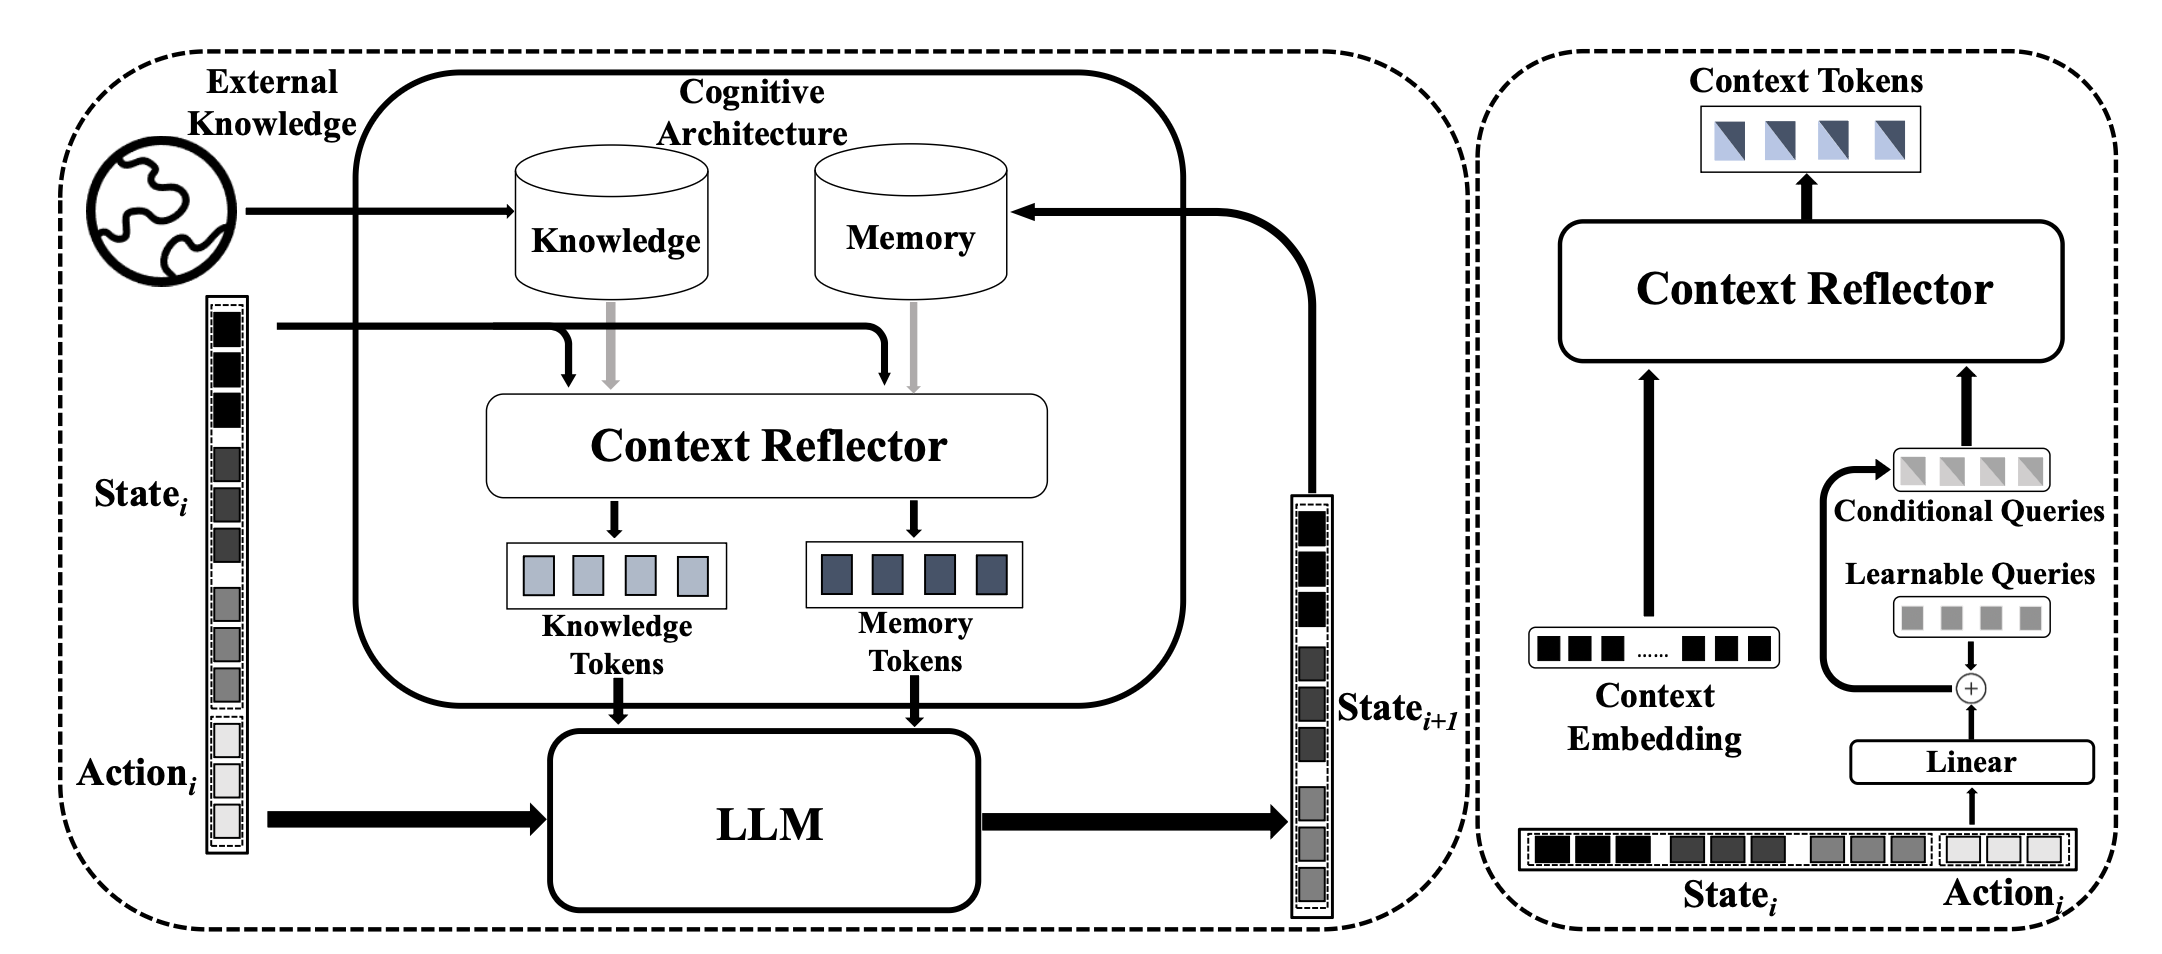
\includegraphics[width=0.95\linewidth]{figures/worldgpt}
    \caption{Architecture of WorldGPT \citep{ge2024worldgpt}}
    \label{fig:worldgpt}
\end{figure}


\paragraph{WorldGPT}
WorldGPT is based on a standard  LLM, Vicuna-7B-v0.\footnote{\url{https://huggingface.co/lmsys/vicuna-7b-v1.3}, \url{https://lmsys.org}} It performs reasoning in latent space, following the model-based reinforcement learning approach. %WorldGPT follows the retrieval-augmented generation (RAG) approach  using external knowledge bases, and also using external (long term) memory, to augment LLM performance further, by addressing the state problem (Section~\ref{sec:state}). 
The goal of WorldGPT is to be a simulator of realistic dynamics of the world---the transition and the reward function in reinforcement learning. To do so, the architecture helps synthesize multi-modal instruction instances, using a special architecture. At the core WorldGPT follows the common VLM architecture with a central LLM, and a multi-modal encoder and a decoder. To help the model synthesize multi-modal instructions, a cognitive architecture is added to help with specialized or long-term tasks. The architecture adds memory, knowledge retrieval, and context reflection. The context reflection is built on Q-former \citep{li2023blip}. See Figure~\ref{fig:worldgpt} for a diagram of the architecture. 

\paragraph{WebDreamer}
WebDreamer is aimed at web-interaction. It distills  a large model, Qwen-70B \citep{bai2025qwen2}, into a small 7B model. The small model is then used for simulating actions with the world model, before acting in the ``real'' web-world. It uses model predictive control (MPC) as planning approach \citep{garcia1989model,schwenzer2021review} for decision making about website actions, re-planning at each interaction step. WebDreamer leverages LLMs  as world model and as value function. The LLM implements
both the simulation function (sim) and the scoring function (score), see Figure~\ref{fig:webdreamer}.
Furthermore, following \citep{koh2024tree}, the LLM is used for candidate action generation (in addition to sim and score). The authors
employ a two-stage approach: first sampling top-$k$ actions, and  
then using the LLM to self-refine unnecessary actions for simulation.

\begin{figure}
    \centering
    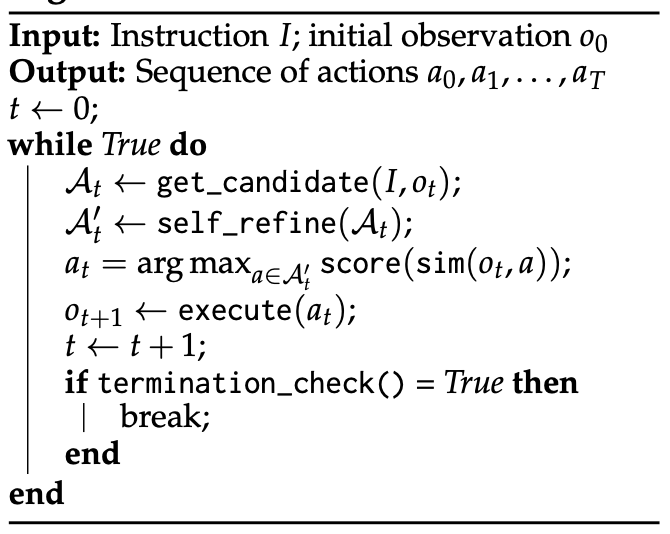
\includegraphics[width=0.5\linewidth]{figures/webdreamer}
    \caption{WebDreamer pseudocode: using LLM for score and sim function \citep{gu2024your}}
    \label{fig:webdreamer}
\end{figure}


\paragraph{WorldCoder}
\begin{figure}
    \centering
    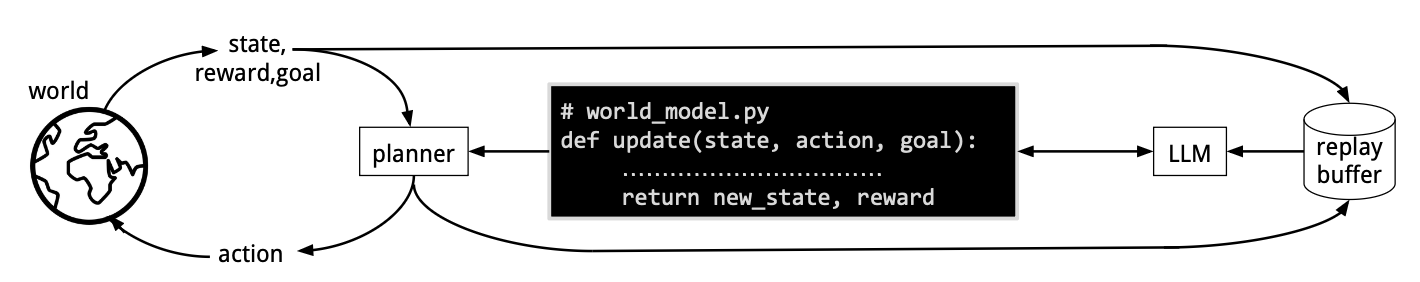
\includegraphics[width=0.95\linewidth]{figures/worldcoder}
    \caption{WorldCoder Architecture \citep{tang2024worldcoder}}
    \label{fig:worldcoder}
\end{figure}
WorldCoder is a model-based agent that builds a Python program to represent its knowledge of the world. WorldCoder creates a transition function of the world in executable Python code, see Figure~\ref{fig:worldcoder}.
WorldCoder uses program synthesis. % It is a model-based agent that builds Python functions to represent its world knowledge. 
In reinforcement learning, problems are formalized as MDPs, consisting of a state representation $S$, action function $A$, transition function $T$, and reward function $R$  (see Section~\ref{sec:mbrl}). WorldCoder uses an LLM to generate Python code for action, transition and reward functions for a task, as well as for the state representation, which is then used in a model-based reinforcement learning approach. This code is   checked and improved, in an iterative self debug refinement process \citep{chen2023teaching}, see Section~\ref{sec:selfdebug}. 
%The  world models are programs, so in each self-debug refinement iteration the LLM is prompted with the erroneous program it previously generated, together with state-action transitions
%that program cannot explain, and prompted to fix its code. 
This process repeats until the program
produces the correct output.

Note that in WorldCoder  the learned model is symbolic (the transition function  is represented as computer code), where in regular deep reinforcement learning the model is a neural network. At inference time, WorldCoder is efficient, since no LLM calls occur that require forward passes through a large network, only interpretation of the transition and reward function Python code.

In regular model-based LLM approaches, the LLM {\em simulates} the world, in WorldCoder the LLM {\em builds} a simulation of the world, for later execution. At inference time, the Python interpreter executes the transition function, where in ReAct, an LLM reasons about the world state. For planning problems, the symbolic approach is better suited, since LLMs struggle with planning during inference (see Section~\ref{sec:knowing}).

\subsection{Learning Algorithm}
We will now discuss the pretraining and finetuning  algorithms that the different approaches use. %Again, a reinforcement learning algorithm is used to learn from feedback.
%RAP  Uses MCTS for planning, with separate prompts for the LLM to use it for the MDP functions.

\paragraph{WorldGPT}
WorldGPT acquires an understanding of world
dynamics by pretraining and finetuning on millions of videos across various domains. Vicuna-7B-v0 is used as the base LLM. Pretraining then uses a language-centric encoder to obtain a unified representation of the multi-modal state. For multi-modal decoding, special tokens are inserted into the LLM's vocabulary. Training starts uni-modal, and progresses to cross-modal.  For finetuning, a special cognitive reinforcement architecture is used with a dataset with fine-grain sequential state-transition sample annotations from more than 10 million videos. As mentioned before, the cognitive architecture consists of memory, knowledge retrieval, and context reflection. Through finetuning, agents  acquire specialized knowledge by finetuning on synthetic multi-modal instruction data.%\todo{wordt er RL gebruikt? PPO?}

\begin{comment}
!!!!!!!!!!!!!!!!!!!!!!!!!!!!!!!!!!!!!!!!!!!!
Ga de papers lezen en schrijf op hoe ze pretraining en finetuning doen.
En check ook architecture!!!!

WebDreamer Summary:
\begin{itemize}
    \item Goal: Be able to use LLM to simulate. Enable Model-based Planning for Web Agents before committing to real action. How can we build effective world models for the Internet? Unlike traditional
world models in RL focusing on improving data efficiency in the agent learning process,
LLM-based world models emphasize decision-making over simulation fidelity, leveraging
broad world knowledge for planning. 
    \item Data: finetune on 3.1 million interaction
instances. Data synthesis pipeline consists of (1) Web Random Walking,
where we autonomously interact with web pages through actions like typing for search
and clicking, and (2) Synthesis, where Qwen2-VL-72B (Wang et al., 2024) generates textual
descriptions of state changes based on visual snapshots before and after actions. 
    \item Arch: LLM as World Model and Value Function. To this end, we introduce WEBDREAMER, a model-based planning framework that uses LLMs to simulate and score possible future states before executing actions. WEBDREAMER leverages LLMs to implement
both the simulation function (sim) and the scoring function (score) (see Figure~\ref{figwebdreamer}).
    \item Learning: Train LLM with scalable data synthesis pipeline. Pretrained on web-scale data, finetune on 3.1 million interaction
instances. Uses MPC which simulates possible
future states for each action over a finite horizon. Implementation
of sim consists of two modules: one predicts
state changes after action execution, approxi-
mating the state transition function T, while the
other imagines a possible action based on the
predicted state to enable long-horizon planning.
Together, these two modules generate trajecto-
ries of length H. Next, use an LLM as a scoring function for each simulation. Furthermore, following \citep{koh2024tree}, LLM is used in addition to sim and score, for candidate action generation. They
employ a two-stage approach: first sampling top-k actions 
then using LLM to self-refine unnecessary actions for simulation.
    \item Results: substantial performance improvements over reactive baselines: 4-5 times more efficient than tree-search. Performance comparable to GPT-4o. competitive with the tree search method, while being 4–5
times more efficient on sandbox environment VisualWebArena, and performs effectively
on real-world websites (Online-Mind2Web and Mind2Web-Live), where tree search meth-
ods are difficult to implement and deploy. Moreover, Dreamer-7B achieves performance
comparable to GPT-4o on two online benchmarks. On Online-Mind2Web and Mind2Web-Live, WEBDREAMER
outperforms the reactive baseline by a relative gain of 42.3\% and 23.8\%, respectively. Another key advantage of model-based planning is its efficiency compared with
tree search using actual explorations. 
\end{itemize}
\end{comment}

\paragraph{WebDreamer} The WebDreamer approach aims to learn  dynamics suitable for model-based reinforcement learning. First the pretrained Qwen-2-VL vision language model \citep{wang2024qwen2} is used to initialize the Dreamer-7B model, which is then further finetuned on 3.1 million interaction examples.
The data synthesis pipeline consists of (1) random walks over the web,
where the model autonomously interacts with web pages through actions such as typing for search
and clicking, and (2) synthesis, where Qwen2-VL-72B  generates textual
descriptions of state changes based on visual snapshots before and after the actions. WebDreamer simulates possible
future states for each action over a finite horizon (replanning and retraining according to the model predictive control (MPC) approach, a reinforcement learning approach for adaptive retraining that is used in  engineering and control problems). 


\paragraph{WorldCoder}
WorldCoder uses program synthesis to learn to make a transition function, the function that computes the next state of the world. WorldCoder then performs planning-actions  using that coded world model. It initially
performs random exploration to initialize a dataset of environmental interactions; it updates its world
model using a program synthesis algorithm, generates the code, and then 
performs planning. Different planners are possible, from    depth-limited value iteration (in
simple domains) to MCTS (for more complex domains) \citep{browne2012survey}.
%combinatorial program synthesis. Explore the space of possible programs.


\begin{comment}
WorldCoder Summary:
\begin{itemize}
    \item Goal: World-coder is a model-based agent that builds a Python program to represent its knowledge of the world, a transition function of the world in executable Python code, see Figure~\ref{fig:worldcoder}. In principle the same knowledge as a regular (non-executable) model, although the WorldCoder model can be run standalone outside a supporting system, and adds options in use and transfer of knowledge. Since WorldCoder can edit its own code, similar to self-reflection in regular (non-executable) models, and it can use this capability to transfer knowledge across environments (generalization). In addition, WorldCoder tries to explain its interactions.

    An important difference between WorldCoder is that the learned model is symbolic (computer code), where in regular deep learning models the model is a neural network. At inference time, WorldCoder is efficient, since no LLM calls occur, just interpretation of the trainsition and reward function code.

    In regular model-based LLM approaches, the LLM simulates the world, in WorldCoder the LLM {\em builds} a simulation of the world, for later execution. At inference time, the Python interpreter executes the transition function, where in ReAct, an LLM reasons about the world state. LLMs struggle with planning during inference, WorldCoder plans easily.
    \item Data:
    \item Arch: an architecture that
synthesizes a Python program to model its past experiences with the world, effectively learning the
transition function
    \item Learning: Learn to make a transition function, the function that predicts the next state of the world. takes actions by planning using that world model. combinatorial program synthesis. Explore the space of possible programs.
    \item Results: world models have many advantages: they allow reasoning in radically new situations
by spending more time planning different actions, and accomplishing novel goals by just changing
the reward function. WorldCoder is tried on gridworlds, and on task planning, finding the approach is more sample-efficient compared to model-free deep reinforcement learning, and more compute-efficient compared to fully-prompt-based ReAct-style agents, and that it can transfer its knowledge across environments by editing its code. 

Sokoban, Minigid, and AlfWorld



Representing world knowledge as code, and generating it from LLMs, brings
other advantages. It allows prior world knowledge embedded in the LLM to inform code generation,
allows sample-efficient transfer across tasks by reusing pieces of old programs, and allows auditing
the system’s knowledge, because programming languages are designed to be human-interpretable.

Though promising, a limitation of the WorldCoder approach is inherent to the computational difficulty of many of the planning problems that it is applied to. Problem instances of combinatorial puzzles such as Sokoban that are difficult to solve with dedicated solvers, will also be difficult to solve for WorldCoder. The transition function that is generated by the LLM is unlikely to be better than those designed by expert human researchers. On the other hand, the LLM may well have seen such codes during pretraining, and the generated transition function may come close, for such problems.

So far, the synthesized  code aims to reproduce the transition and reward functions. Self reflection and metalearning approaches may be able to improve performance further.
\end{itemize}
\end{comment}

%Different planners are suggested for WorldCoder, such as depth-limited value iteration (in simple domains) and MCTS (for more complex domains).




\subsection{Results}
We will now look at the results of the three approaches. 
%RAP works on planning blocksworld, math question answering.

\paragraph{WorldGPT} The WorldGPT model is evaluated with a multi-modal state transition prediction benchmark. WorldGPT is effective, and understands and predicts the dynamics of complex real-world kitchen and cooking scenarios accurately. 
%of  real-life scenarios. Evaluations
%on WorldNet directly demonstrates WorldGPT’s capability to accurately model state transition patterns, 
%affirm its effectiveness in understanding and predicting the dynamics of complex scenarios. 

The system is also evaluated as a world simulator, showing that %the synthesis of multimodal instructions allows 
it can generalize to unfamiliar domains.
In one experiment, WorldGPT is 30 times faster then traditional diffusion-based methods  on audio-video question answering
tasks \citep{ge2024worldgpt}.

\paragraph{WebDreamer} WebDreamer also performs well. It is reported to surpass GPT-4o performance on web interaction tasks.
Substantial performance improvements are reported over reactive baselines, on which it is 4-5 times more efficient than tree search. WebDreamer performs well  on the sandbox environment VisualWebArena, and also on real-world websites (Online-Mind2Web and Mind2Web-Live), where tree search methods are difficult to implement and deploy. Moreover, on online benchmarks, using Dreamer-7B, the approach achieves performance
comparable to GPT-4o. On real-world websites, WebDreamer
outperforms the reactive baseline with a relative gain of 42\% and 24\%, respectively. %Another key advantage of model-based planning is its efficiency compared with tree search using actual explorations. 

\paragraph{WorldCoder} 
For WorldCoder  results are reported on grid worlds and on task planning (AlfWorld). WorldCoder is more sample-efficient than model-free reinforcement learning, and more compute-efficient compared to ReAct-style agents that try to perform in-context planning by the LLM. %, and that it can transfer its knowledge across environments by editing its code.

% The WorldCoder system assumes deterministic dynamics and requires symbolic state representations. WorldCoder is tried on gridworlds, and on task planning, finding the approach is more sample-efficient compared to model-free deep reinforcement learning, and more compute-efficient compared to fully-prompt-based ReAct-style agents, and that it can transfer its knowledge across environments by editing its code. 
% Sokoban, Minigid, and AlfWorld

Generating world knowledge as computer code by LLMs brings
advantages. It allows prior world knowledge embedded in the LLM to improve code generation, as existing solutions to published problems may well have been seen during pretraining. The code can also be transferred across tasks by reusing pieces of old programs. Furthermore, the results are human readable, allowing the world knowledge to be inspected by humans by reading the generated code.
%auditing the system’s knowledge, because programming languages are designed to be human-interpretable.

Though promising for planning problems, a limitation of the WorldCoder approach is inherent to the computational difficulty of planning problems. Problem instances that are difficult to solve with dedicated solvers are also difficult to solve for WorldCoder solvers. The transition function that is generated by the LLM is unlikely to be better than those designed by expert human researchers. %On the other hand, the LLM may well have seen such codes during pretraining, and the generated transition function may come close, for such problems.

So far, the synthesized  code aims to reproduce the transition and reward functions. For future work, self reflection and metalearning approaches may be able to improve performance further.



\subsection{*Model-Based Reinforcement Learning}\label{sec:mbrl}




\begin{comment}
    
World models have  been studied  in reinforcement learning, before they became popular in LLMs. It is useful to discuss briefly the type of world models that have been created in that field. 
%World models have been studied in reinforcement learning, before they became popular in LLMs. 
To better understand the background of world models, we will start our discussion with a discussion of world models in reinforcement learning, the so-called {\em model-based} reinforcement learning.

Reinforcement learning is a method to learn a policy of the best actions for the states that an agent can be in. Reinforcement learning is an online learning method, actively uncovering the data that it learns from, at training time (in contrast to supervised learning, that needs a preexisting data set that must be prepared offline). For reinforcement learning, the policy starts empty, and the policy is improved online, as new feedback comes in. Turning back to our topic, Agentic LLM, in reinforcement learning terms, Agentic LLMs are  model-free reinforcement learners that learn the best actions online, as they are interacting. However,  Agentic LLMs do not start empty, they use a large and expensively pretrained language model, an offline model, and thus this online learning process can only be a part of the picture. 

In addition to the model-free online learning process for the policy, reinforcement learning can also learn its own model, a {\em dynamics model}, of the world. This so-called {\em world model}  contains a condensed and efficient representation of the environment in which it operates, that can be easily and efficiently accessed by the agent, without having to interact with the world.


%From a reinforcement learning perspective, an Agentic LLM can be seen simply building a world model in a model-based reinforcement learning design. The dynamics model is represented 
\end{comment}
World models are being used successfully in agentic LLM. An extensive literature exists on world models in model-based reinforcement learning. At the end of this chapter, we will now provide a brief overview of world models in model-based reinforcement learning, in order to provide more context for the use of world models  in LLM. 

An influential early model-based approach is Dyna \citep{sutton1991dyna}. Influential recent works are \citep{ha2018world,hafner2020mastering}. Two modern surveys  are \citet{moerland2023model,plaat2023high}.

In reinforcement learning, agents learn how to act in an
environment by sampling rewards from actions that are executed in the environment. % (see Figure~\ref{fig:rl7}). 
%
%
% \begin{figure}
%   \begin{center}
%     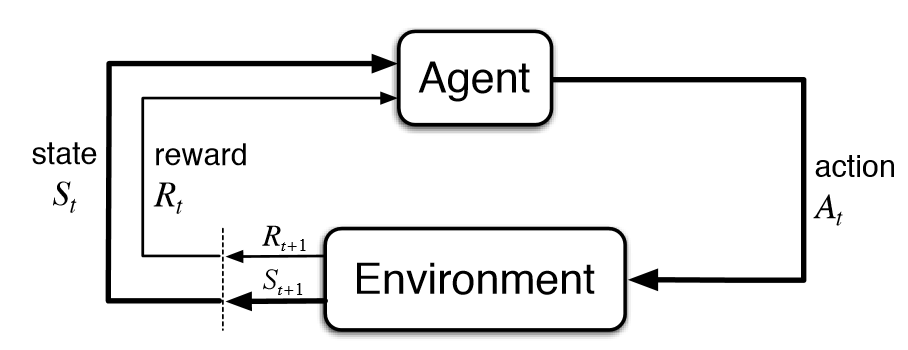
\includegraphics[width=9cm]{figures/rl}
%     \caption{Reinforcement Learning: Agent acting in Environment \citep{sutton2018reinforcement}}\label{fig:rl7}
%   \end{center}
% \end{figure}
%


%World models have been successful in learning robotic movement in complex environments, to play Atari video games, and to act in open world games such as MineCraft \citep{hafner2020mastering,hafner2023mastering}.
%World models can also be
%trained effectively with LLMs \citep{ge2024worldgpt}. 
%For example, WorldCoder builds a world model as a Python program from
%interactions with the environment \citep{tang2024worldcoder}. The world model explains its
%interactions with a language model.

%Make a new model, to use as input, new training data.

%While world models are mostly associated with reinforcement learning,
%they are also used to generate a model in planning domains (blocks-world) in PDDL, to aid task-planning \citep{guan2023leveraging},
%achieving success in ALFWorld \citep{shridhar2020alfworld}.


% Can VLAs help take actions?
%Agents can learn a policy to act with reinforcement learning from surrogate world models. However, agents can also learn action models directly. 
%
%New models to train on.
%Three examples are
%\citet{ahn2022can,radford2021learning,suglia2021embodied}, who ground
%language models in world models of robotic actions. 
%\citet{xiang2024language} use world models to finetune language models
%to gain diverse
%embodied knowledge while retaining their general language capabilities.




%Connection between inference time planning and learning world model. Planning as outerloop Metalearning?


\begin{figure}
  \begin{center}
    \input figures/rl
    \caption{The standard reinforcement learning loop. The agent learns a $\theta$-parameterized policy $\pi_\theta$ from feedback rewards $r$ from the environment. \citep{sutton2018reinforcement}}\label{fig:rl7b}
  \end{center}
\end{figure}

\subsubsection{Model-free Reinforcement Learning}
In regular reinforcement learning an optimal agent policy  is learned model-free: the best actions for all states are learned directly from interaction with the environment (see Figure~\ref{fig:rl7b}), without the help of an extra model of the environment. Regular reinforcement learning is formally described as a Markov decision process, with four functions $\{S, T, A, R\}$: a function $S(o)\rightarrow s$ to represent the state of the system for observation $o$, a function $T(s,a)\rightarrow s'$ that transitions from one state to the next state using an action, a function $A(s)\rightarrow a$ that returns an action for a state, and a function $R(s)\rightarrow r$ that assign a reward value (positive or negative) to a state. The goal of reinforcement learning is to use the MDP to learn an optimal policy $\pi^*(s)\rightarrow a^*$, the function that returns the best action for each state that the MDP can be in. Thus, a reinforcement learning problem consists of four functions $S$, $T$, $A$, and $R$, and the goal of the agent is to find the optimal policy $\pi^*(s)$ with the highest expected cumulative reward. The agent does not have access to $T$ and $R$, functions that reside in the environment. %If the agent wants to know if action $a$ is a good action, the so-called {\em policy evaluation} problem, then it has to perform action $a$ in the environments, which uses $T$ to transition to new state $s'$ and $R$ to compute the reward value $r$ of that new state, and return $(s', r)$ to the agent. The agent then uses $r$ to update the value for the action in the policy, the so-called {\em policy improvement} step.
Regular, model-free, reinforcement learning is also called {\em direct} reinforcement learning. %The agent samples that environment, and improves the policy with feedback on each action. 
The direct method naturally has high sample complexity: policy improvement requires sampling, and large MDPs require many samples for the policy improvement process to converge (Figure~\ref{fig:rl7b}). 

%Now, when the real environment is too complex, executing those actions in the real environment may be too expensive, and learning the policy takes too long. In that case, agents may learn an extra, smaller, world model as a surrogate, locally. Accessing this local surrogate model is assumed to be cheap. They can then use this local model of the dynamics of the world to allow sample efficient training of the policy.  Such local world models are learned on the fly by model-based reinforcement learning from the environment interaction, concurrent to policy learning. Thus, each environment sample updates both the policy $\pi$ and the local model $M=(T', R')$.

\begin{figure}[ht]
  \begin{center}
    \input figures/mbrl
    \caption{Model-based reinforcement learning where environment feedback is used to improve both the policy $\pi$ and the local dynamics model $\hat{M}=(\hat{T},\hat{R})$ from which the policy $\pi$ is also sampled ({\em planning})}\label{fig:mbrl}
  \end{center}
\end{figure}

\subsubsection{Model-based Reinforcement Learning}
In direct reinforcement learning, sampled information is not retained by the agent, but forgotten, and each policy improvement requires a new sample.  Interaction by the agent with the outside environment is often expensive, for example for a robot acting in the real world, whose joints wear out. In this case it would be beneficial to find ways to reduce the sample complexity. We should try to improve the policy without having to sample as much from the environment. 

A straightforward idea is not to throw away the samples, but to store them in a buffer, and also sample from that buffer of older interaction results, or, slightly more advanced,  to train a {\em local surrogate model} $M=(\hat{T}, \hat{R})$ of the environment dynamics. When we have trained this local dynamics model, we can also sample from the model, cheaply, in addition to sampling the environment, expensively (see Figure~\ref{fig:mbrl}). 

These methods are indirect methods, since, in the last methods, where a local dynamics model is built up by the agent, the policy is learned indirectly (through a local model) from the environment. 

Using a local dynamics model is called model-based reinforcement learning. The dynamics model consist of local estimations  $\hat{T}$ and $\hat{R}$ by the agent, estimates of the real $T$ and $R$ that are known only to the environment. 
Model-based reinforcement learning has been successful in some applications, such as Go \citep{silver2016mastering}, Diplomacy \citep{meta2022human}, StarCraft \citep{vinyals2019grandmaster}, and showing learning across domains \citep{hafner2020mastering}. 


Model-based reinforcement learning  also connects to {\em planning}, a classic field in symbolic artificial intelligence, that looks ahead into the future, simulating different possible worlds using the efficient latent representation, without having to act in the real world. 

\subsubsection{Dimension Reduction}
In deep model-based reinforcement learning, the local dynamics  models  are also called world models \citep{ha2018world}. 
In this context world models reduce high dimensional observation spaces to lower dimensional state and reward spaces, that can then be used in model-based reinforcement learning methods to efficiently improve policy functions. 
%, that sample from the low-dimensional dynamics model.
The idea
behind world models is that in most high-dimensional environments
there are elements that are less important, such as, in a video game, trees in the  background 
that never move,  that have little or no relation to the value
of the agent's actions. The goal  is to
abstract away these  unimportant elements of the input space, 
reducing the effective dimensionality of the state space.

\subsubsection{Joint Embedding Predictive Architecture}
The joint embedding predictive architecture (JEPA) is proposed by \citet{lecun2022path} and further refined in \citet{assran2023self}. The goal of JEPA is to predict future states in an abstract, compressed representation (latent space) rather than trying to recreate raw sensory details or pixels. This goal is similar to the dimension-reduction goal of a world model in model-based reinforcement learning. Where model-based reinforcement learning uses learns a local transition model supervised by rewards, JEPA is a self-supervised representation learning framework. 
JEPA is trained  via self-supervised observation (watching videos or images) to map context embeddings to target embeddings without rewards or explicit actions. Model-based reinforcement learning explicitly incorporates actions, rewards, and control optimization to maximize the return \citep{lim2026jedi}. JEPA and reinforcement learning are close, JEPA can be used as a perception engine (world model) for reinforcement learning or planning algorithms, for example to guide robotic control \citep{destrade2025value}.


\begin{comment}
!!!!!!!!!!!!!!!!!!!!!!!!!!!!!
En nu world model gaan noemen. En dat een LLM een world model is, en met fine tuning online verbeterd wordt door interactie. ICRL kan dan samplen van het world model (het LLM) om de optimale policy te bepalen. acties.

\todo{Sectie herschrijven. Er is nog geen lijn. Eerst logische lijn maken} The agent improves its policy of best actions for each state from the reward that an outside environment provides, see Figure~\ref{fig:rl7}. After using the reward for updating the policy, it is thrown away, and new rewards are sampled from the environment. This model works when environment interaction is cheap, but when it is expensive, then it might be more advantageous to remember the rewards, and have the agent build its own model of the environment, from which the agent can then also take (cheap) samples to as it is improving its policy function. This approach is called model-based reinforcement learning \citep{moerland2023model,plaat2023high}, and it has been successful in some applications, such as Go \citep{silver2016mastering}, Diplomacy \citep{meta2022human}, StarCraft \citep{vinyals2019grandmaster}, and showing learning accross domains \citep{hafner2020mastering}. The locally learned models learn the transition function and the reward function. Together, they are  called the dynamics model, since it models the dynamics of the environment. The models are also called world models. World models are an important factor in the success of agents. 


 Recall that the environment
samples return $(s',r')$ pairs when the agent selects action $a$ in
state $s$. This means that  we can learn the
transition model $T_a(s,s')$ and the reward model $R_a(s,s')$, for
example by supervised learning, since
all necessary information is present. When the transition and reward model are
present in the agent, they can then be  used with planning to update
the policy and value functions as often as we like \emph{without any
  further sampling of the environment} 
(although we might want to continue sampling to further improve our
models). This
alternative approach  
of finding the policy and the value is called model-based learning,
see Algorithm~\ref{lst:back} and Figure~\ref{fig:learn}. 


\begin{figure}[t]
  \centering
    \input figures/learn
    \caption{Model-Based Reinforcement Learning}\label{fig:learn}
  
\end{figure}




\begin{figure}[t]
  \begin{center}
    \input figures/imagination
    \caption{Dyna's Model-Based Imagination}\label{fig:imagination}
  \end{center}
\end{figure}



%
%
\begin{algorithm}[t]
  \begin{algorithmic}
    \Repeat
    \State Sample env $E$ to generate data $D=(s, a, r', s')$ 
    \State Use $D$ to learn $T_a(s,s')$ and  $R_a(s,s')$ 
    \State Use $T, R$ to update policy $\pi(s, a)$ by planning 
    \Until $\pi$ converges
  \end{algorithmic}
  \caption{Model-Based Reinforcement Learning}\label{lst:back}
\end{algorithm}

% If the model is given, then no environment samples are needed and 
% model-based methods are  more sample efficient. But if the
% model is not given,
Why would we want to go this convoluted learning-and-planning route,
%which may even introduce model-bias,
if
the environment samples can teach us the optimal policy and value directly? The
reason is that the convoluted route may be more sample efficient.

In model-free learning
a sample is used once to optimize the policy, and then thrown away,
while in
model-based learning 
the sample is used to learn a transition model, which can then be used many
times in planning to optimize the policy. The sample is
used more efficiently by the agent.
 
A well-known classic model-based approach is \emph{imagination}, which was
introduced by~\citet{sutton1990integrated,sutton1991dyna} 
in the Dyna system, long before deep learning was used widely. 
%Dyna uses the environment samples to update the policy  function directly (model-free learning) and also uses the samples to learn a transition model,  to augment the model-free environment-samples with the model-based imagined ``samples.'' % In this way the sample-efficiency of model-free
% learning is improved quite directly.
%Imagination is a hybrid algorithm that uses both model-based planning and model-free learning to improve the behavior policy.
% , with the creation of these imagined planning updates.
%Figure~\ref{fig:imagination} illustrates
%the working of the Dyna approach.
%Algorithm~\ref{lst:dyna} shows the
%steps of the algorithm (compared to  Algorithm~\ref{lst:back}, the
%line in italics is new, from Algorithm~\ref{lst:free}). Note how the
%policy is updated twice in each iteration, by environment sampling, and by
%transition planning. More details are shown in Algorithm~\ref{alg:dyna-q}~\citep{sutton1990integrated}.


\begin{algorithm}[t]
  \begin{algorithmic}
    \Repeat
    \State Sample env $E$ to generate data $D=(s, a, r', s')$ 
    \State {\em Use $D$ to update policy $\pi(s, a)$}
    \State Use $D$ to learn $T_a(s,s')$ and  $R_a(s,s')$ 
    \State Use $T, R$ to update policy $\pi(s, a)$ by planning 
    \Until $\pi$ converges
    \end{algorithmic}
    \caption{Dyna's Model-Based Imagination}\label{lst:dyna}
\end{algorithm}

% Dyna was introduced for a tabular approach before deep learning
% became popular. In Dyna,  the transition model is updated directly
% with samples.
%Note that the policy network is now updated twice in each iteration,
%once with 
%environment samples, and once with the  planning data.
%

% learn the policy without direct environment
% samples for the policy. In Dyna  the model-free lookahead planning is
% called ``imagination.'' In contrast to the previous section, in Dyna
% the same method is used for optimizing the policy
% from real experience as from imagined experience, generated by planning.






\begin{algorithm}[t]
  \input figures/dynaq
  \caption{Dyna-Q: Classic learning and planning with a Q-function-based dynamics model~\citep{sutton1990integrated}} 
  \label{alg:dyna-q}
\end{algorithm}

The principles of Dyna have been developed further in various directions, which we will now discuss.




%\subsection{World Models !!TOTAL REWRITE!!}
\todo{No, essence of world models is not high dimensionality, essence is a local copy of the environment to learn more efficiently from. Talk about planning (Dyna) and then Dreamer}
A major challenge in machine learning that has been addressed by deep learning is to model high dimensional problems. In reinforcement learning, World models do so in model-based reinforcement learning. 
%\todo{Yes, but in model free also deeo learniing} 
World models reduce high dimensional observation spaces to lower dimensional state and reward spaces, that can then be used in model-based reinforcement learning methods to efficiently improve policy functions, that sample from the low-dimensional dynamics model.
The idea
behind world models is that in most high-dimensional environments
there are elements that are less important, such as background trees
that never move,  that have little or no relation with the reward
of the agent's actions. The goal  is to
abstract away these  unimportant elements of the input space, 
reducing the effective dimensionality of the space. 
%!!!!!!!!!!!!!!!!!!!!!!
World models do so by
learning the relation between the elements of the input and the
reward  either by auto encoding or with supervised learning
conditioned on value.  %When we focus our learning mechanism  on the changes in observations that are correlated with changes in these values, then we can improve the efficiency of  learning high-dimensional problems greatly.
%Unimportant elements (such as background trees that never move) have
%a weak relation with the reward, and they are abstracted away.
World models thus learn a smaller representation, smaller than the
observation space.
Planning  takes place in this smaller representation space.



% It turns out that in high-dimensional input scenes
% typically only a few objects influence the reward, and many elements
% are irrelevant. 
% Think of images of landscapes in which a character
%moves, where trees in the background do not influence the score, or
%images of a robot-arm, where a desk  in the background never
%moves, and similarly does not influence the reward of the action to
%be learned.


%In an early example of world models, the  value prediction network (VPN), introduced by ~\citet{oh2015action,oh2017value}, 
%to achieve this goal. They 
%ask the question in their paper: ``What if
%we could predict future rewards and values directly without predicting
%future observations?'' and 
%describe a network architecture and learning
%method for models focused on value prediction. The core idea is not to
%learn directly in actual observation space, but 
%first to
%transform the actual state representation to a smaller latent representation
%model, also known as abstract model. 
%The other functions, such as
%value, reward, and next-state, then work with the smaller latent representations,
%instead of the actual high-dimensional states. By training all functions based on the
%values, planning and learning occur in a space
%where states are encouraged only to contain the elements that influence
%value changes. % Non-essential elements, such as trees, houses, or other
% unchanging background, are not part of the latent states.
%We will now explain the latent-model approach using VPN.\footnote{See
%  \url{https://github.com/junhyukoh/value-prediction-network} for the code.}
%In VPN the world model consists of four networks: an (LSTM) encoding
%function, a reward function, a value function, and a transition
%function. All functions are parameterized with their own set of
%parameters (Figure~\ref{fig:oh}).
%
%Latent space is lower-dimensional, and training and planning become more efficient.
%The figure shows a single step rollout, planning one step ahead, 
%as in Dyna-Q (Algorithm~\ref{lst:dyna}).

% To distinghuish these latent-based functions from the
% conventional observation-based functions $R, V, T$ we denote them
% differently as $f^{enc}_{\theta_e}, f^{reward}_{\theta_r},
% f^{value}_{\theta_v}, f^{trans}_{\theta_t}$.

% \begin{itemize}
% \item The encoding function $f^{enc}_{\theta_e}:s_{actual}\rightarrow
% s_{latent}$ maps the observation $s_{actual}$ to the abstract state
% using a neural network $\theta_e$, such as a CNN for visual observations.
% \item The latent-value function
%   $f^{value}_{\theta_v}:s_{latent}\rightarrow
%   V_{\theta_v}(s_{latent})$ maps the abstract state to its value using
%   a separate neural network $\theta_v$. This value is the value of the
%   latent state, not of the actual observation state $V(s_{actual})$.
% \item The latent-reward function $f^{reward}_{\theta_r}:(s_{latent},o)\rightarrow r,
% \gamma$ maps the latent state and option (a kind of action) to the
% reward and discount factor. If the option takes $k$ primitive actions,
% the network should predict the discounted sum of the $k$ immediate
% rewards as a scalar. (The role of options is more fully explained in the paper.) The network also predicts option-discount factor
% $\gamma$ for the number of steps taken by the option.
% \item The latent-transition function $f^{trans}_{\theta_t}:(s_{latent},o)\rightarrow
%   s'_{latent}$ maps the latent state  to the next latent state,
%   depending also on the option.
% \end{itemize}
% Figure~\ref{fig:oh} shows how the function work together, with $x$ the
% observed actual state, and $s$ the encoded latent
% state~\citep{oh2017value}. 



 %\begin{figure}[t]
 %\begin{center}
 %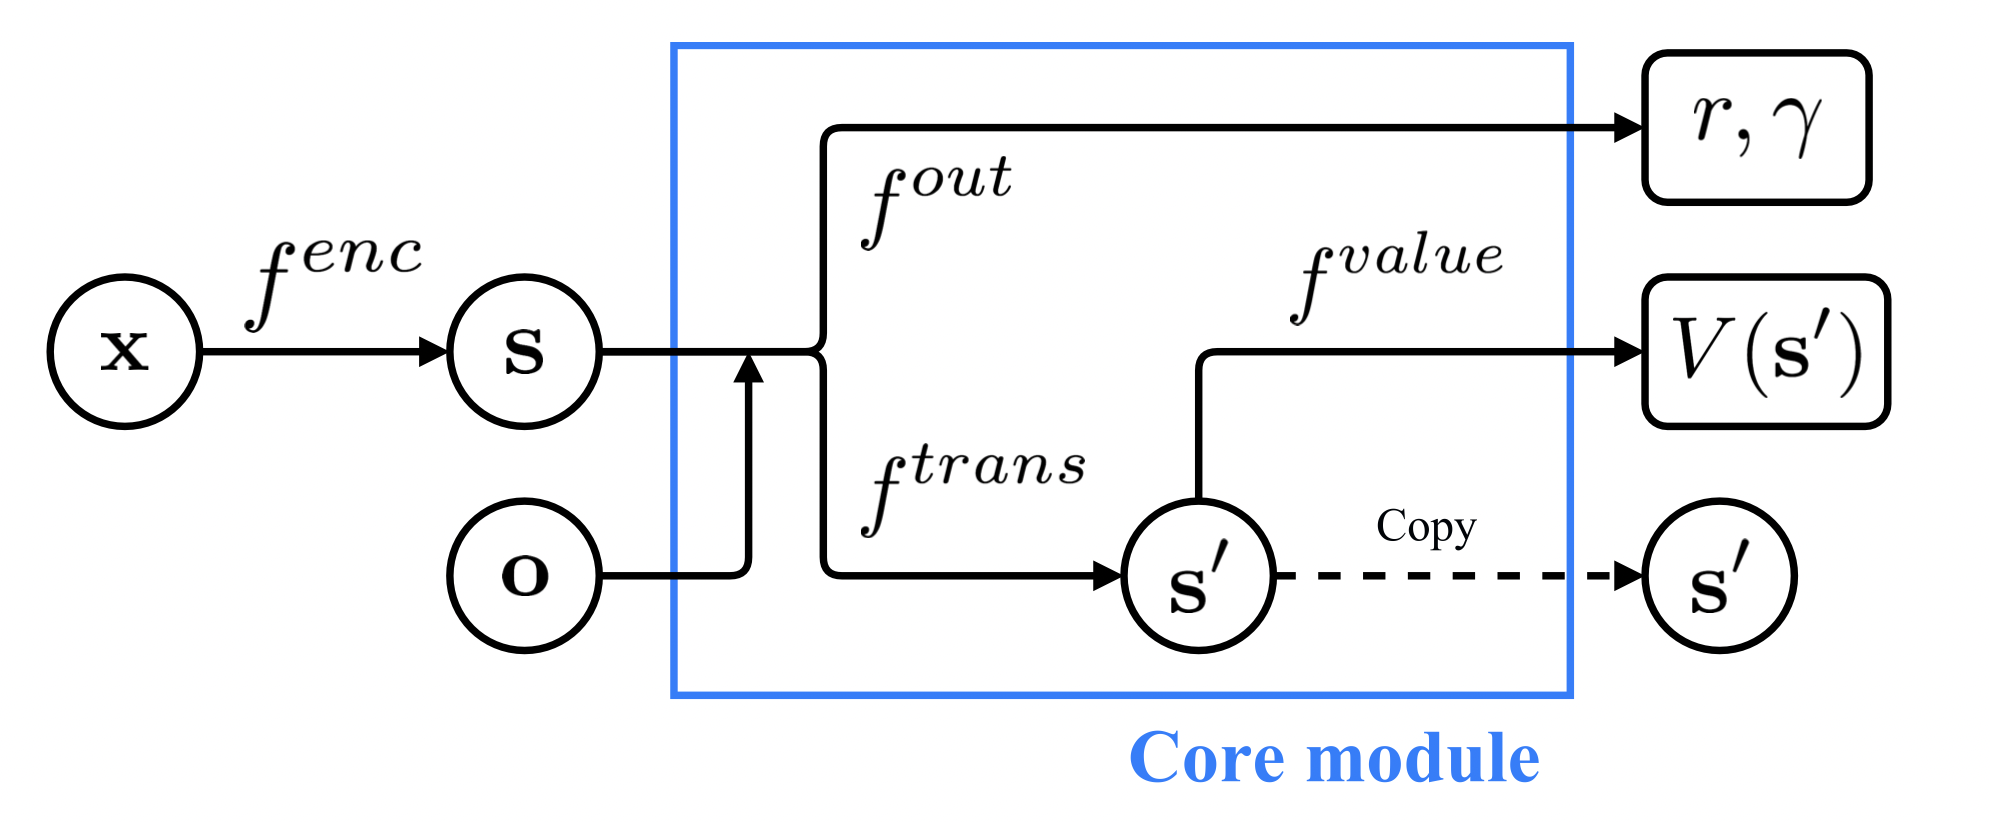
\includegraphics[width=7cm]{figures/oh2017core}
 %\caption{Architecture of world model VPN~\citep{oh2017value}}\label{fig:oh}
 %\end{center}
 %\end{figure}


% , where the model was used for
% single step sampling, just as the environment. Howerver, in contrast to an
% environment, a model also allows looking further into the future, by
% performing multi-step rollouts. Of course, this requires a highly
% accurate model, otherwise the accumulated inaccuracies diminish the
% value of the far-into-the-future lookahead. Algorithm~\ref{alg:dplan}
% shows the pseudocode for a $d$-step planner for the value prediction
% network.
% % \footnote{
% %The Q-value in the pseudocode is calculated as
% %$Q_\theta^d(s,o)=r+\gamma V^d_{\theta}(s')$ where
% %$V^d_\theta(s)=\frac{1}{d}V_\theta(s)+\frac{d-1}{d}\max_o
% %Q_\theta^{d-1}(s,o)$  and if $d=1$ then $V_\theta^d(s)=V_\theta(s)$.}



% \begin{algorithm}

%   \begin{algorithmic}
%             \Function{Q-Plan}{s, o, $d$}
%             \State  $r, \gamma, V(s'), s' \rightarrow
%             f^{core}_\theta(s, o)$ \Comment{Perform the four latent functions}
%             \If{$d=1$}
%             \State \Return{$r+\gamma V(s')$}
%             \EndIf
%             \State $A\leftarrow b$-best options based on $r+\gamma
%             V_\theta(s')$ \Comment{See paper for other expansion strategies}
%             \For{$o'\in A$}
%             \State $q_{o'} \leftarrow $ Q-Plan$(s',o',d-1)$
%             \EndFor
%             \State \Return{$r+\gamma[\frac{1}{d}V(s')+\frac{d-1}{d}\max_{o'\in
%                 A} q_{o'}]$}
%         \EndFunction
%   \end{algorithmic}
%   \caption{Multi-step planning~\citep{oh2017value}}\label{alg:dplan}

% \end{algorithm}

%The training of the networks can in principle be performed with any
%value-based reinforcement learning algorithm. \citet{oh2017value} report results
%with $n$-step Q-learning and temporal difference search~\citep{silver2012temporal}.
%In
%general, trajectories are generated with an $\epsilon$-greedy policy
%using the planning algorithm from Algorithm~\ref{alg:dplan}.
%VPN~\citep{oh2017value} showed impressive results on Atari games such as Pacman
%and Seaquest, outperforming model-free DQN~\citep{mnih2015human}, and outperforming
%observation-based planning in stochastic domains.
%Subsequently, many other works have been published that further
%improved
%results~\citep{kaiser2019model,hafner2018learning,hafner2019dream,hafner2020mastering,sekar2020planning,silver2017predictron,ha2018world}.
%Many of these world-model approaches are complicated designs, with
%multiple neural networks, and different learning and planning algorithms.



% {\bf 
% Dit moet beter, dit is niet te volgen en vaag. Het gaat er om om
% algemene principes uit te leggen.
% } 

%In the next section we will discuss the performance of latent models.
In an influential early work, ~\citet{ha2018world} describe how world models are inspired
by the manner in which humans are thought to construct a mental model of
the world in which we live. Originally, world models were often
represented as recurrent neural networks that were trained using a variational
autoencoder~\citep{kingma2013auto,kingma2019introduction,goodfellow2014generative}. Later, transformer architectures were used, that were trained self-supervised. 
%They  learn a compressed spatial and temporal
%representation of the environment. In world models  multiple neural
%networks are used, for  a vision model, a
%memory model, and a controller~\citep{ha2018world}. By using features extracted from
%the world model as inputs to 
%the agent, a compact and simple policy can be trained to solve a
%task, and planning occurs in the compressed or simplified world. World
%models have been applied by~\citet{ha2018recurrent,ha2018world} on a
%car racing game~\citep{kempka2016vizdoom}.
The term
\emph{world model} %actually 
goes back to 1990~\citep{schmidhuber1990making}. 
%Latent models are  related to dimensionality
%reduction~\citep{van2009dimensionality}.
%Some ideas have to wait a
%long time before their time has come.

%{\bf is there a large sample complexity reduction?}



% The role of latent models in image-based reinforcement learning can be
% compared with the attention mechanism in natural language processing.
% In natural language processing the concept of attention has been quite
% important. Attention~\citep{sutskever2014sequence,cho2014learning} uses
% an encoder-decoder RNN mechanism  to improve the performance  machine
% translation.   Together with the
% subsequent development of transformer models, attention has caused breakthrough
% results such as the large language models GPT-2 and
% 3~\citep{devlin2018bert,radford2018improving,radford2019language,brown2020language}. 



% {\bf dit verhaaltje hieronder is fout, de crux is niet dat het meerdere functies zijn, maar dat het een compactere representatie van de observaties is}

% Latent models are born out of this need for
% more accurate predictive deep models. Latent models replace the
% single transition model with separate, smaller, specialized, representation models,
% for the different functions in a reinforcement learning algorithm. All
% of the elements of the MDP-tuple  may now get their own
% model. Planning occurs in latent space.


% Traditional deep learning  models represent
% input states directly in a single model: the layers of neurons and filters are all
% related in some way to the input and output of the domain, be it an
% image, a sound, a text or a joystick action or arm movement. All of
% the MDP functions, state, value, action, reward, policy, and discount, act on
% this single model. Latent models, on the other hand, are not connected
% directly to the input and output, but are connected to other
% models and signals. They do not work on direct representations, but on
% latent, more compact, representations. The interactions are captured in three to four
% different models, such as observation, representation, transition, and
% reward models. These may be smaller, lower capacity, models. They may be trained with
% unsupervised or self-supervised deep learning such as variational autoencoders~\citep{kingma2013auto,kingma2019introduction} or
% generative adversarial networks~\citep{goodfellow2014generative}, or recurrent networks.
% Latent models use multiple
% specialized  networks, one for each function to be
% approximated.



% Figure~\ref{fig:abstract} illustrates the abstract (latent) learning
% process (using the modules of 
% Dreamer~\citep{hafner2019dream}  as an example).
% %
% \begin{figure}[t]
%   \begin{center}
%     \input abstract
%     \caption{Latent Models}\label{fig:abstract}
%   \end{center}
% \end{figure}

% \subsubsection{CNN}
% Only in the context of e2e, of a network to learn the transition
% function, and at the same time the planning function

% {\bf En wat moet ik hier dan vertellen???}
The architecture of world models is elaborate. The
dynamics model typically includes an observation model, a
representation model, a transition model, and a value or reward
model~\citep{karl2016deep,buesing2018learning,doerr2018probabilistic}. 
%The task of the observation model is to reduce the
%high-dimensional world into a lower-dimensional world, to allow more
%efficient planning. Often a (variational) autoencoder or LSTM is used. 
%
%The Arcade learning environment is one of the main benchmarks in
%reinforcement learning. The 
%high-dimensionality of Atari video input has long been problematic for
%model-based reinforcement learning. Latent models were instrumental in
%reducing the dimensionality of Atari, producing the first successes
%for model-based approaches on this major benchmark.

%Related to the VPN approach~\citep{oh2015action,oh2017value} are
%latent model approaches, such
%as~\citet{kaiser2019model}, that are aimed at video prediction,
%outperforming model-free baselines~\citep{hessel2017rainbow}, reaching
%comparable accuracy with up to an order of magnitude better sample
%efficiency. The approach by~\citet{kaiser2019model} uses a variational
%autoencoder (VAE) to process input frames, conditioned on the actions of the
%agent, to learn the world model, using PPO~\citep{schulman2017proximal}. The policy $\pi$ is then improved by planning inside the
%reduced world model, with short rollouts. This behavior policy $\pi$ then determines the
%actions $a$ to be used for learning from the environment.

%Latent models are also used on continuous MuJoCo problems. 
The
work by~\citet{hafner2018learning,hafner2019dream} on the PlaNet and
Dreamer systems is
noteworthy. They  include the
application of their work back to Atari~\citep{hafner2020mastering},
which achieved human-level performance.
PlaNet uses a Recurrent state space model (RSSM) that consists of a transition model, an observation model, a variational
encoder and a
reward model~\citep{karl2016deep,buesing2018learning,doerr2018probabilistic}. %{\em Planner:}
%Based on these models a Model-predictive control agent
%is used to adapt its plan, replanning each
%step~\citep{richards2005robust}. The RSSM is 
%used by a Cross entropy method search (\citet{botev2013cross}, CEM)  for the best action
%sequence. %~\citep{karl2016deep,buesing2018learning,doerr2018probabilistic}.
%In contrast to model-free approaches, no explicit policy or value
%function network is used; the policy is implemented as MPC planning
%(see next section)
%with the best sequence of future actions. PlaNet is tested on
%continuous tasks and reaches performance that is close to
%strong model-free algorithms.

A further system, called
Dreamer~\citep{hafner2019dream}, builds on PlaNet. 
%Using an actor
%critic approach~\citep{mnih2016asynchronous} 
%and backpropagating value gradients through predicted sequences of compact
%model states, the improved system  solves a diverse collection of
Dreamer is used on continuous problems from the Deepmind control
suite~\citep{tassa2018deepmind}, see Figure~\ref{fig:dcs}. Dreamer is also applied to discrete 
problems from the Arcade learning environment, and to few-shot
learning~\citep{sekar2020planning}. 
A further improvement 
achieved human-level performance on 55 Atari games, a first for a
model-based approach~\citep{hafner2020mastering}, showing that the
latent model approach is well-suited for high-dimensional problems.

% , solving At  and discrete control tasks.
% - more complex ocntrol tasks/DCS, also atari
% - backprop value gradients through imagined trajectories through latent model, actor critic
% - build on planet, better performance than planet. learning a value
% model in imagination enables Dreamer to solve long-horizon tasks while
% being robust to the imagination horizon. 

% PlaNet is used on MuJoCo. So is Dreamer. RSSM:VAE


%Schmidhuber
\paragraph{Planning}
Planning algorithms are the cornerstone of classic artificial intelligence, to search a space of possible states. The Monte Carlo Tree Search algorithm does so efficiently, and without the need for guidance from   heuristic.
%\todo{Op dit punt echt volslagen onduidelijk waarom MCTS er bij moet. Heel anders brengen. Uitleggen dat het gebruikt wordt in LLM prompting} 
Since its invention in 2006 \citep{coulom2007monte,kocsis2006bandit} as a search algorithm for the game of Go, it has been remarkably successful in a wide range of applications \citep{browne2012survey,plaat2020learning}.   

\end{comment}

\subsubsection{Agentic World Models}
In the context of model-based reinforcement learning, LLMs can be used in two different ways. We can use a pre-trained (static) LLM as world model $(\hat{T}, \hat{R})$ in model-based reinforcement learning (LLM4MBRL). Often this approach uses a tree search or MCTS planning. In this approach, the LLM is used to help reinforcement learning. 

Alternatively  (model-based) reinforcement learning settings can be used to train LLM world models (MBRL4LLM) with feedback from world-interaction. Now, the LLM has become adaptive, either through an adaptive harness, or by posttraining the model itself, as in a VLA. 
This approach is also known as agentic world models,
and holds much promise for agents to better understand their environment, to act in more realistic ways. In this approach, reinforcement learning is used to help agentic language modeling.  This is an active area of research, see, for example, 
\citet{zuo2026qwen}, including their references.\footnote{There is a third connection between reinforcement learning and language modeling. Model-free reinforcement learning is also used {\em inside} the LLM training pipeline, for finetuning, as in RLHF and RLVR.}  %\todo{Dit misschien eerst dan} 


%Summarize. There are so many combinations of planning and world models and MBRL. All very much agent-like. MBRL/World Model might well be the Agentic LLM architecture.

%Perhaps a separate section on what to use on what circumstance?

%How? By approach or by technique?



\begin{comment}
    
\section{Decision Transformers}\todo{weg? vergelijk met wat er in 6.2.4 en 6.2.6.3 allemaal al staat} !!!!!!!!!!!!!!!!!!!!!!!!!!!!!
VLAs can be pretrained for robotic action on visual information, and world models provide important information for agentic decision making. 

In this section, we will focus on sequential decision making, and look at yet a new type of model:  decision transformers.
Many artificial intelligence applications can be modeled as sequential decision making processes, where to reach a goal, we need to make the right intermediate steps (think of playing chess, or preparing a cappucino: one wrong move, and you get a mess). 
Agentic models  need decision models to act in the world.
Solutions can be learned online (reinforcing on feedback, from an environment)---with conventional neural networks, and offline (under supervision, from datasets)---with transformer models.  


Note that the models in this section are not pretrained LLMs, but the raw transformers. In this section the  transformers are not pretrained on language, but  on decision traces. The goal in this section is not to speak a natural language, but to see if we can capture the essence of decision making in our models. The central learning method in this section is  not self-supervised learning, but reinforcement learning. The transformers in this section are not trained on language, they are not LLMs. The purpose of this  section is to find out if  transformers can make decisions, and how. 

Decision making involves evaluation of prompts to find the answer, it involves generation of new prompts and exploration of  alternatives, and it involves backtracking, to keep track of which options have been tried and which are still to be explored. For decision making, an implicit tree of options is searched. In the previous chapter we have seen that LLMs and transformers have no problem in  generating and evaluating prompts, but that they do not manage state well, and, hence, backtracking will be difficult. In-context learning solved this problem by using external algorithms to perform the backtracking. In this section we will see which architectural solutions have been devised to pretrain an LLM for decision making, and how the pretrained decision transfomers work synergistically with inference time algorithms such as ICRL. This section is the finetuning version of Tree of Thoughts, without the language part.

%has developed methods to solve such applications successfully. 
%Since the transformer architecture is also an effective method for sequence modeling, solving the next-token-prediction problem very effectively, a natural question is to see if transformers work well in sequential decision problems, can a transformer be pretrained on decision sequences?

%Moet dit verhaal? 
%VLM is  een LLM but pretrained on new visual data.
%Past hier mooi, in dit Pretrain hoofdstuk
First we will discuss the tasks that decision models are solving.

\subsection{Tasks}
The decision tasks that these models are trained on are often the familiar benchmarks from in-context learning:  math word, question answering, and the smaller reinforcement learning MDP tasks. 

Among the math word problems are GSM8K \citep{cobbe2021training}, AIME24 \citep{codeforcesamerican}, MATH500 \citep{hendrycks2021measuring}. 
Question answering tasks include StrategyQA 
\citep{geva2021did}, 
Big Bench Hard \citep{srivastava2023beyond}.
Small reinforcement learning problems include Multi-armed bandits and contextual bandits \citep{lu2010contextual}, CartPole \citep{sutton2018reinforcement}, and 2D and 3D navigation tasks such as Miniworld \citep{MinigridMiniworld23}.
Puzzles and games include Game of 24 \cite{yao2024tree}, Mini Crosswords \citep{yao2024tree}, Tic Tac Toe, Chess, and Hex. 

The tasks range from easy (GSM8K, CartPole, Bandits) to hard (AIME, Chess), and are useful to study different questions in the field. We will now discuss different architectures which are used for decision models.

%These are all benchmarks that are tested and well understood.

%decision models for agents are diverse, and range from boards games, to robotics, and locomotion.

%vorig hoofdstuk al genoemd dat decision transformers gepretrained kunnen worden. Schulz, Lee hebben dat gedaan. Met search traces, en wat meer?

%In tegenstelling tot ICRL, hier worden models zelf op decisions getrained.
%Wat zijn de taken?
%Games, robots, locomotion, action in real world.
%Lookup the list of applications from 
%Schulz: Chess, Chess960, Connect Four, Hex
%Demircan: MDP Two step task, Grid world, 
%Schmied, MABandits, Contextual bandits, Tic Tac Toe
%Lee, MABandit, Dark Room 2d Grid, Mini World 3D navigation, 
%Li, math word problem benchmarks, AIME, QA, BBH
%Guo, AIME, MATH500
%Sel, Game of 24, Mini Crosswords, GSM8K, Strategy QA
%Wang CartPole


%Othello, Hex, Chess, Diplomacy, BALROG, Robot, Locomotion



\subsection{Architecture}
The VLM architecture combines two kinds of static data, using two kinds of encoders. It used self-supervised learning on two different static data types, images and Language. Both supervised learning from static dataset.




\subsection{Learning Algorithm}
Transformers can be trained on decision sequences from the start of the training pipeline, at pretraining time. They can be trained on decision states only, giving a decision-only model, or also on language, giving a decision-language model. 

Decisions can also enter the training pipeline at a later stage, at finetuning time. In this case our model is pretrained as a regular language model, and then finetuned on decisions. 

We will discuss both approaches, and start with pretraining pure transformers that are trained on decision sequences.

Pretraining for language and images uses self-supervised learning:  Take a large corpus and do masked next word prediction. With decision making, reinforcement learning is used, where the model generates (CoT) prompts and answers dynamically, that are compared against an external reward function. This may be a quick function, for example, GRPO uses the form of the answer, without checking in detail whether the content is correct.

An advantage of reinforcement learning is that training data are generated dynamically, on demand, until either the training accuracy has improved sufficiently, or when a computational resource limit has been reached.

Inference time follows action and computes new state and reward. New state and reward must be used for finetuning. So we need RLFT. Title of section could be: "from SFT to RLFT." Aha! Found the new storyline!! So the architecture is unchanged transformers, but the training algo has gone from SFT to RLFT.
And the interpretation from the transformers has changed from next token to next state, which is perhaps close enough.

A story line that studies TD, pretraining search traces, finetuning on CoT rationales, which is also what GRPO does I think, AoT multiple pathways encoding.
Difference between pretraining an empty transformer, and finetuning an LLM. 




%Architecture:
%SDP->Transformer

%\subsubsection{Pretraining Decisions from Scratch}


\subsubsection{Pretraining Transformers on Decision Sequences}
%Dus: Pretraining


Basically: Supervised on database of decisions


\paragraph{DPT} Supervised pretraining on offline dataset of state/action pairs
Lee DPT
to allow a range of problems to be solved in context, showing online exploration



 
\paragraph{TD} 
Demircan finds evidence of TD-error values in model after prompted for traces, ICRL shows TD errors in the model.  (No pretraining, only SAE for understanding ICRL)
\paragraph{search traces} Schulz pretrain txf on search traces, with decision trees. Find that Txf can be trained to perform tree search. 
Nog eens lezen. Leert het model echt zoeken? Echt backtrack?


Also: Othello, Hex \citep{schultz2024mastering}.
Pretrain on Internal search. 
Compare to external search. 
It partly works.
%Learning (sequences from scratch):
%Pretraining:

Wang Transformer (not LLM) can be pretrained for TD learning in forward pass (at inference time). Needs ICRL at inference time. Pretraining the model to be ready for ICRL at inference time. Mostly theory paper with proofs.

\paragraph{Implicit reasoning}
In addition to external reasoning algorithms, there is also recent work on Implicit reasoning \citet{li2025implicit}. Implicit reasoning adapts transformer architectures to allow them to reason internally, without the need for an external prompt-optimizing algorithm. For example, it uses extra latent embeddings and neural
network layers. Implicit reasoning is the name of a group of methods. They all require a new network architecture, which has to be pretrained. Implicit reasoning thus holds the promise of a more elegant architecture (not needing an external algorithm to patch shortcomings of transformers) and more efficiency (no need for many expensive calls at inferences time for each new thought or variable state). The disadvantage is of course that each new network architecture has to be pretrained from scratch.  \todo{REWRITE} Three paradigms for implicit reasonign are: (1) Latent optimization focuses on directly manipulating the internal representations without generating explicit textual steps. (2) Signal-Guided Control uses specialized input signals to steer internal computation without producing intermediate textual outputs. (3) Layer-Recurrent Execution introduces recurrence into the transformer's forward pass, allowing multi-step reasoning through repeated processing. Implicit reasoning is an active area of research, discussing the methods in detail is outside the scope of this book. For an excellent overview, see \citet{li2025implicit}.
%\todo{Is this an architecture? Is this %Pretraining? Finetuning?} It is a new architecture, certainly having to be pretrained. on Language??? LLM???


%\subsubsection{Finetuning RLFT}


\subsubsection{LLM Decisions: Finetuning LLMs on decision sequences}
Dus: Finetuning

DeepSeek? Methods: RLHF, PPO, DPO, GRPO

\citep{demircan2024sparse,schmied2025llms,krishnamurthy2024can}

%Finetuning (sequences RLFT):
\paragraph{CoT rationales} Schmied RL finetuning on self-generated CoT rationales. finetuning enhances the decision-
making abilities of LLMs by increasing exploration and narrowing the knowing-doing gap. Like DeepSeek but for decision making. During RLFT the model learns to iteratively refine its reasoning process,
favoring CoT patterns and actions that lead to higher rewards.
Pipeline of RL on top of LLM, which has standard architecture.
\paragraph{GRPO} 
\citep{guo2025deepseek} introduced the DeepSeek finetuning method, a method that used only reinforcement learning to finetune the model, greatly benefiting the efficiency of the finetuning stage. The DeepSeek approach also integrates Chain of Thought reasoning thoughts, further improving efficiency of the fine tuning. The DeepSeek-Zero model was finetuned, on the base model, just by reinforcement learning, without any extra data, using the  GRPO finetuning algorithm. 
\paragraph{AoT} 

Sel AoT encode a pathway across multiple options in a single CoT prompt, encode choice in the prompt. This is not pretraining at all. This should go to previous chapter, as an enhanced form of CoT, single prompt. Maaaaar: in sectie 5 doen ze ook een finetuning experiment, en dat laat goede resultaten zien. Ook hier is het de interplay tussen inference time en trainign time, uiteinedleijk. Dit AoT kan in H6 en in H7. Kiezen.
Toch weer een mooi voorbeeld van combinatie van inference time en training time.
Should finetune with CoT thoughts. Als DeepSeek.
AoT os LLM, not just transformer, but on top of pretrained LLM (GPT4)
%\paragraph{ICRL}

%Orden de text hieronder volgens de structuur hierboven




%\todo{So, what's the story? How can transformers learn to choose and backtrack, or is it they learn the single best option based on input? Re-read Schulz. Policy is single option per state. Transformer large enough to hold entire state space? Then the transformer is one big policy network. Then pretraining could work.}
 

%Very different
%Hmm. is dat zo? Moet het noodzakelijkerwijs alleen maar at inference time? Zou een model zelf niet het kiezen kunnen leren? Als CoT?
%I mean, Schulz shows that LLMs can be pretrained on searches. Inferencing decisions, forward pass does choice? 










\subsection{Results}

Tsja, wat zijn de resultaten? Hoe goed werkt het?
Wel... DeepSeek doet het enorm goed, en efficient, ook op klein netwerk. Math, en verder?
What kind of applications?

DeepSeek-R1-Zero, DeepSeek-R1. DeepSeek achieved state of the art performance on a wide range of regular and reasoning LLM applications: advanced math word reasoning (AIME and MATH500), computer code (Codeforces and SWE-bench), question answering (GPQA Diamond), and language understanding (MMLU).

Algorithm of Thought achieved good results on decision making/reasoning tasks (Game of 24 and Mini Crosswords), both with finetuning and without finetuning (ICRL).

In the games of Chess and Hex encouraging results were achieved by pretrainging the decision transformer on minimax \citep{markeeva2024clrs,knuth1975analysis,plaat1996research} and MCTS \citep{browne2012survey} search traces \citep{schultz2024mastering,kempinski2025game}. Other works report encouraging results in the game of Othello \citep{li2023emergent,kempinski2025game,chen2025if}. 

Implicit reasoning is currently an active field of research, for results, see the literature \citep{li2025implicit}.

\end{comment}

\section{Concluding Remarks}
%The transformer architecture is a versatile architecture. With the attention mechanism it finds correlations between tokens. When trained on large datasets, it becomes quite good at next-token prediction, and when the dataset is very large, in-context few-shot learning emerges. Especially on sequence data, transformers work well.

Transformers can be trained on tokenized language data, but also on other tokenized data. In this chapter we have seen different model architectures for different modalities. Architecturally, the models were quite different.  However, most models are transformer based, and tokenization approaches have been devised for a surprising difference in modalities.  Let us review the different types of models to see what they have in common:
\begin{itemize}
    \item  Large language models (LLM) are transformers that are pretrained on {\em tokenized natural language}.
    \item Vision language models (VLM) are models that consist of a transformer that is trained on {\em tokenized vision data} (or a diffusion model, or a convolutional network) and a transformer trained on {\em tokenized natural language}, whose embeddings come together in a joint decoder.
    \item Decision transformers (DT) are transformers that are trained on {\em tokenized $(s,a,r)$-episodes} of decision paths (see Section~\ref{sec:decisions}).
    \item Vision language action models (VLA) are models that consist of a vision-language architecture that are also trained on {\em tokenized $(s,a,r)$ episodes} of robotic actions.
    \item World models are models that consist of a vision-language architecture that are also trained on {\em tokenized $(s,a,r)$ episodes} of real world actions or decisions. 
\end{itemize}
There are other types of models that we have not discussed in this chapter. For example, a large music model (LMM) is a transformer that is pretrained on tokenized musical sequences (which can be either symbolic music (score sheets) or a soundtrack) \citep{yuan2025yue}.

This chapter was devoted to advanced models for agents. We discussed language models that were pretrained and finetuned on vision and action. These models understand more of the world, allowing agents to achieve impressive generalization results. We have seen how the LLM, originally a language model, is becoming a world model, a term that is borrowed from the field of model-based reinforcement learning. 

At this point it might be good to look back on what we have seen so far.
The first part of the book explained how to {\em pretrain} models self-referentially for {\em language}. Then, Chapter~\ref{chap:reasoning} explained how {\em in-context learning} emerged, and how it can be used for inference time  {\em multi-step reasoning} and self-reflection. This chapter discussed {\em pretraining} and {\em finetuning} methods to yield {\em multi-modal world} models of the environment. Together, pretrained language, inference time reasoning, and finetuned world models enable agents more and more to act intelligently and achieve tasks in the world for their users. %\todo{Dus het gaat over world models in dit hoofdstuk. Niet zozeer over decision transformers. Dat was meer de finetuning insteek. Dus 7.4 kan weg. Het reasoning/CoT gedeelte is al in H6 behandeld. Al dat Schultz gedoe met games is teveel mijn hobby} 

We have now discussed many different modalities and training methods. In the next chapter we will take a step back and reflect on  how agents can learn in a stable manner, while they are also acting in the world that they learn from.


\bibliographystyle{plainnat}
\bibliography{agenticbook,refs,case,synthetic}


%Pretraining, Finetuning  models for agentic actions. VLM, VLA, World models, Decision Transformers. The developments of models specifically designed for action taking is continuing. 

%In the next chapter, we will look at agent architectures, and at metalearning. Metalearning describes the learning processes of active agents well.
%
%\subsubsection{RAP. Just Model-free ICL. Uses static World Model}
%\citep{hao2023reasoning} LLM planning with MCTS: RAP
%
%\paragraph{Goals:}
%Do reasoning better on challenging goals: blocksworld, math, question
%answering.
%
%RAP leans on Planning, blocks world, also to claim importance of results, since LLM do not do blocks world well.
%\paragraph{Architecture:}
%MCTS with LLM as world model, using prompts for the different
%functions of MDP: T/A/R
%Standard LLM: LLaMa or GPT4, with different prompts to specify the MDP
%role T/A/R.
%\paragraph{Learning Algorithms:} ICL
%\paragraph{Pseudo Code:}
%MCTS code from paper
%Copy the algorithm 1 RAP-MCTS Appendix
%\paragraph{Results:}
%Results are good. Copy the Blocksworld, GSM8K, QA tables.
%
%Conclusion. So we can use an LLM as the elements of a RL/MDP. Using
%MCTS to take care of state in problems that need state (blocksworld),
%and tree shape state space search. RAP uses LLM for MDP functions as
%in a regular model-free RL design. Not like a world model from MBRL.
%So they have good results, sure, but it is not an MBRL-dreamer style
%worldmodel. The LLM does not learn, it is fixed. It is more like the
%environment, than like a learning local dynamics model. It is a
%pretrained static LLM whose parameters do not change. So what is the
%nature of a world model? it is the model-free environment. Just like
%the ToT, but than with an MCTS instead of DFS. And a nice fancy
%name. World Model. Like AlphaZero. But now with an LLM instead of a
%ResNet. And using natural language, much easier to setup than
%AlphaZero, which needed many many years of design.
%
%Confusing terms. Model Free RL has an Environment. No World
%Model. ModelBased RL has a World Model. RAP does model free, or MCTS,
%to be precise. We could also just call it evaluation function. Toch
%wel een beetje oude wijn in nieuwe zakken en de keizer die geen kleren
%heeft. Maar wel mooie experimentele resultaten.
%
%Doet dit nu Pretraining/Finetuning? Nee. HEt hoort dus in H6, niet H7.
%Well. That was quick.
%This is a prime example of an ICRL implementation.
%Should just mvoe to Ch6. Really.  
%
%Well, it uses a model of the world. Just a static one, pretrained on general knowledge. Not specifically online on the environment. But the LLM is a model that it uses for planning. So maybe it is MBRL after all? Offline????
%
%\paragraph{Summary:}
%MCTS on top of LLM, in order to manage state
%understanding the world. Although they stress that MCTS is important
%for Exploration/Exploitation balance, I think it is especially
%important to keep track of world state.
%
%So. LLM is used as world model for all the different functions of the
%MDP, which is then planned over by MCTS, which does that very well,
%because MCTS is good in planning. Works well for the applications
%Blocksworld, GSM8K, Question Answering.
%
%Models used:
%LLaMa-33B, GPT4
%
%Application domains:
%Blocksworld, GSM8K, PrOntoQA
%
%LLM as reasoning agent=$\pi$: $\pi(s,c)\rightarrow a$: given s, the
%LLM as reasoning agents, given prompt c,  generates a
%
%LLM as world model=$T$: $T(s,a,c')\rightarrow s'$: the LLM as world model
%generates next state s with another prompt to generate the next state
%
%LLM as reward model=$R$: $R(s)\rightarrow r$: the LLM generates a
%reward for the  state; or use task specific heuristics, or log
%probability of action as likelihood of reward

